\chapter{Tense and aspect constructions 2: narrative markers}
\is{narrative markers|(}\is{narrative|(}
\label{NarrativeMarkers}
\section{Introduction}
\is{narrative tense|(}\is{subsecutive|(}
This chapter deals with two verbal paradigms whose use is essential for understanding coherent narrative discourse in Nyakyusa: the narrative tense (\sectref{NarrativeTense}) and the subsecutive (\sectref{Subsecutive}). \tabref{TableNarrativeMarkers} shows the formal composition of the two.

\begin{table}[H]
\begin{center}
\begin{tabular}{llll}
\lsptoprule
\footnotesize{Label} & \footnotesize{Shape} & \footnotesize{Example}\\
\midrule
Narrative tense & \textsc{sm}-\textit{lɪnkʊ}-\textsc{vb}-\textit{a} & \textit{tʊlɪnkʊjoba} & \lq we spoke' \\  
Subsecutive & \textsc{sm}-\textit{a}-\textsc{vb}-\textit{a} & \textit{twajoba} & \lq (then) we spoke'\\
\lspbottomrule  
\end{tabular}
\caption{Narrative markers}\label{TableNarrativeMarkers}
\end{center}
\end{table}

In the following sections, first a short approximation to the concept of narrative markers will be given, together with an overview over the commonalities and differences between Nyakyusa's two narrative markers (\sectref{NarrativeMarkersComparison}). This is followed by an in-depth examination of the the narrative tense and the subsecutive (\sectref{NarrativeTense}, \ref{Subsecutive}).

\section{The two narrative markers: a comparison} \label{NarrativeMarkersComparison}

\label{NarrativeMarkersApproximation}
Dedicated narrative markers are a common device in African languages \citep[113f]{DahlOe1985}. Concerning Bantu, \citet{NurseD2008} gives a rough description of what makes up this wider category:

\begin{quote}
The time of the situation is first established, either explicitly in the first verb in a string, or implicitly [\ldots] All following verbs in the sequence are then marked by a special narrative marker, which replaces the tense marker appropriate to the time established by the first verb. Just because most sequences deal with past events, this special marker is most frequent in past narratives, less frequent in timeless events, followed by futures. It also occurs across sentences and utterances, in which case the context most often crosses sentence boundaries and characterizes a long utterance. Use of the special marker can be suspended and then deliberately reintroduced by the speaker to stress continuity.  \citep[120]{NurseD2008}
\end{quote}

Nurse's description will serve as a valuable starting point for an understanding of the function of narrative markers in Bantu. Nevertheless, it contains a number of points that require further scrutiny as they relate to the Nyakyusa narrative tense and subsecutive. Before turning to a closer examination of these points for each of the two narrative makers, some more general points about the Nyakyusa inventory of narrative markers are worth a discussion.

To begin with, \citet[120]{NurseD2008} goes on to generalize that ``most [Bantu] languages have only one narrative marker and the number of narrative markers never exceeds that of past tense markers.'' Nyakyusa, having two narrative markers, thus not only runs counter to a strong tendency within the language family, but contradicts Nurse's second generalization, as Nyakyusa does not make remoteness distinctions in the past.\is{tense!past}\footnote{Unless one classifies the present perfective\is{aspect!perfective} as a near past,\is{tense!past} an attribute that rather derives from its more general aspectual meaning (\sectref{PresentPerfective}).}

In the following sections, common typologies of narrative markers will be discussed (\sectref{NarrativeMarkersTypologies}), to then take a closer look at the pragmatic factors that license the employment of the Nyakyusa narrative markers (\sectref{NarrativeMarkersLicensingDependency}). This is followed by a discussion of their distribution in the macro-structure of narrative discourse (\sectref{NarrativeMarkersUseDistribution}) and their quantitative distribution (\sectref{NarrativeMarkersQuantitativeDistribution}). Lastly, \sectref{NarrativeMarkersFunctionalDifferences} summarizes the functional differences between the two narrative markers.

\subsection{On typologies of narrative markers}\label{NarrativeMarkersTypologies}
Given Nyakyusa's inventory of two narrative markers, the question arises as to how far they differ in meaning and use. In discussions of narrative markers, especially for African languages, two typologies are commonly encountered. The first one has a syntactic\is{syntax} basis and distinguishes narrative markers according to the subject of the verb thus marked \citep[19]{RoseEtal2002}. Narrative markers that are used with the same subject as that of the initial verb then classify as \textit{consecutive} or \textit{narrative}. A narrative marker used with different subjects, on the other hand, is termed a \textit{subsecutive}/\textit{sequential}. However, \mbox{(dis-)}continuity of the grammatical subject is not a delimiting parameter in Nyakyusa. Firstly, both the Nyakyusa narrative tense and the subsecutive can co-occur in the same stretch of a narrative, as in (\ref{exSubsecutiveJaKufikaRepetitionEnda}) below. Secondly, the subject of both the narrative tense and the subsecutive may be the same as that of the initial verb within a span; see e.g. (\ref{exNARRhoboka}) below for the narrative tense and (\ref{exSubsecPigDuck}) for the subsecutive. Both are, however, also found with different subjects; see e.g.(\ref{exNARRhoboka}) below for the narrative tense and (\ref{exSubsecAfterIPFVFelbergstory}) for the subsecutive. %XXX anderes BSP different subject NARR
\is{storyline ranks|(}
Another dichotomous typology of narrative markers has been proposed by \citet{LongacreR1990}, who focuses on pragmatic factors. He distinguishes a \textit{narrative tense}, defined as marking only storyline events (i.e. only those events that advance the narrative) and possibly used from the first clause of a text onwards, from a \textit{consecutive tense}, which is ``either dependent on a special initial form and/or is rank-shifted in sequence with non-storyline initials'' \citep[109]{LongacreR1990}. The first criterion, dependency on an initial form, will be examined in  \sectref{NarrativeMarkersLicensingDependency}.

Longacre's second criterion, rank-shifting, deserves a short excursion. In his work on narrative discourse, Longacre stipulates that in any given language there is a verbal construction associated with those clauses that advance the progress of a story. Once this construction is identified, the remaining verbal paradigms or constructions used in narrative discourse can be ranked. This ranking is based on the degree that the clauses they are found in depart from the main storyline (e.g. secondary storyline > backgrounded actions > setting). Some languages may also posses a construction that is used in those clauses that rank higher than the main storyline (pivotal events). \is{storyline ranks|)}
\subsection{Licensing and dependency}\label{NarrativeMarkersLicensingDependency}
As discussed in \sectref{NarrativeMarkersTypologies}, \citeauthor{LongacreR1990}'s (\citeyear{LongacreR1990}) typology distinguishes between those narrative markers that can be used from the first clause of a narrative on and those that require the employment of an initial verb form.

An examination of the text corpus shows that all narratives open with at least one past tense verb, typically in the form of an orientation section\is{section!orientation} that may vary in length. Thus in (\ref{exNARRopeningSentence1}), not only the protagonists are introduced, but the situation is established by the use of the past imperfective.\is{aspect!imperfective}\is{tense!past} The onset of the storyline here coincides with the use of the narrative tense (\ref{exNARRopeningSentence2}, \ref{exNARRopeningSentence3}).

\begin{exe}
	\ex \label{exNARRopening}
	\begin{xlist}
		\ex \label{exNARRopeningSentence1} \gll po leelo ɪ-m-bwele \textbf{j}-\textbf{aa}-\textbf{lond}-\textbf{aga} ʊkʊtɪ jɪ-j-eeg-e ɪ-m-bʊlʊkʊtʊ\\
		then now/but \textsc{aug}-9-mosquito 9-\textsc{pst}-want-\textsc{ipfv} \textsc{comp} 9-9-marry-\textsc{subj} \textsc{aug}-9-ear\\
		\glt `So, Mosquito wanted to marry Ear.'
		\ex \label{exNARRopeningSentence2}\gll po leelo ɪ-m-bwele \textbf{jɪ}-\textbf{lɪnkʊ}-\textbf{bʊʊk}-\textbf{a} kʊ-m-bʊlʊkʊtʊ\\
		then now/but \textsc{aug}-9-mosquito 9-\textsc{narr}-go-\textsc{fv} 17-9-ear\\
		\glt `So Mosquito went to Ear.'
		\ex \label{exNARRopeningSentence3}\gll \textbf{jɪ}-\textbf{lɪnkʊ}-\textbf{tɪ} \textup{\lq\lq}gwe, m-bʊlʊkʊtʊ, ʊ-ne n-gʊ-gan-ile fiijo \ldots\textup{''}\\
		9-\textsc{narr}-say \phantom{\lq\lq}\textsc{2sg} 9-mosquito \textsc{aug}-\textsc{1sg} \textsc{1sg}-\textsc{2sg}-love-\textsc{pfv} \textsc{intens}\\
		\glt `It said ``You, Ear, I love you very much \ldots''{}' [Mosquito and Ear]
	\end{xlist}
\end{exe}

Note that while in the case of (\ref{exNARRopening}) the onset of the storyline coincides with a shift from a past tense\is{tense!past} verb to the narrative tense, this is not true for all texts. This will be discussed in detail in \sectref{NarrativeMarkersUseDistribution}.

To continue, negative data corroborates the observation that neither the narrative tense nor the subsecutive can by themselves open a text. Constructed mini-narratives that open with a verb in the narrative tense, such as (\ref{exNARRFromFirstClause}), were unanimously rejected by the language assistants and corrected so as to start with a past tense verb (\ref{exNARRFromFirstClauseCorrected}). Note that this example does feature the frame adverb \textit{mmajolo} \lq yesterday'.

\begin{exe}
	\ex\label{exNARRFromFirstClause}
	\begin{xlist}
		\ex[\#]{\gll m-ma-jolo \textbf{n}-\textbf{dɪnkʊ}-\textbf{lembʊk}-\textbf{a} n=ʊ-lʊ-bʊnjʊ fiijo\\
			18-6-evening \textsc{1sg}-\textsc{narr}-awake-\textsc{fv} \textsc{com}=\textsc{aug}-11-morning \textsc{intens}\\}
		
		\ex[]{\gll n-dɪnkʊ-nw-a ɪɪ-t͜ʃai\\
			\textsc{1sg}-\textsc{narr}-drink-\textsc{fv} \textsc{aug}-tea(9)(<SWA)\\}
		
		\ex[]{\gll bo n-nw-ile ɪɪ-t͜ʃai n-dɪnkʊ-bʊʊk-a kʊ-kʊ-kam-a ʊ-lʊ-kama \ldots\\
			as \textsc{1sg}-drink-\textsc{pfv} \textsc{aug}-tea(9) \textsc{1sg}-\textsc{narr}-go-\textsc{fv} 17-15-milk-\textsc{fv} \textsc{aug}-11-milk\\
			\glt (intended: \lq Yesterday I got up very early. I had breakfast (lit. \lq drank tea'). When I finished breakfast, I went to milk the cows …') [ET]}
	\end{xlist}
	\ex\label{exNARRFromFirstClauseCorrected} Correction of (\ref{exNARRFromFirstClause}):
	\begin{xlist}
		\ex[]{\gll m-ma-jolo \textbf{n}-\textbf{aa}-\textbf{lembwike} n=ʊ-lʊ-bʊnjʊ fiijo\\
			18-6-evening \textsc{1sg}-\textsc{pst}-awake.\textsc{pfv} \textsc{com}=\textsc{aug}-11-morning \textsc{intens}\\}
		\ex[]{\gll n-dɪnkʊ-nw-a ɪɪ-t͜ʃai \ldots \\
			\textsc{1sg}-\textsc{narr}-drink-\textsc{fv} \textsc{aug}-tea(9)\\}
	\end{xlist}
\end{exe}

Constructed texts whose opening sentence consists of a temporal clause\is{subordinate clauses!temporal clause} referring to a specific situation, such as (\ref{exNARRFromFirstClauseWithAdverbial}), however, were accepted.
\begin{exe} %specific situation ist zwar schwamming, aber das soll Becker sagen
	\ex \label{exNARRFromFirstClauseWithAdverbial} \begin{xlist}
		\ex \gll m-ma-jolo, \textbf{bo} \textbf{n}-\textbf{gʊ}-\textbf{pɪlɪk}-\textbf{a} ɪɪ-ng'ombe si-kʊ-jweg-a fiijo \textbf{n}-\textbf{dɪnkʊ}-\textbf{lembʊk}-\textbf{a}\\
		18-6-evening as \textsc{1sg}-\textsc{prs}-hear-\textsc{fv} \textsc{aug}-cow(10) 10-\textsc{prs}-shout-\textsc{fv} \textsc{intens} \textsc{1sg}-\textsc{narr}-awake-\textsc{fv}\\
		\glt `Yesterday, when I heard the cows making a lot of noise, I got up.'
		\ex \gll n-dɪnkʊ-bʊʊk-a kʊ-kʊ-kam-a ʊ-lʊ-kama \ldots\\
		\textsc{1sg}-\textsc{narr}-go-\textsc{fv} 17-15-milk-\textsc{fv} \textsc{aug}-11-milk\\
		\glt `I went to milk the cows …' [ET]
	\end{xlist}
\end{exe}

The same can be observed for the subsecutive: constructed mini-narratives such as (\ref{exSubsecutiveFromFirstClause}) were rejected by the language assistants and corrected so as to start with a past tense verb\is{tense!past} (\ref{exSubsecutiveFromFirstClauseCorrected}).

\begin{exe}
	\ex\label{exSubsecutiveFromFirstClause}
	\begin{xlist}
		\ex[\#]{\gll m-ma-jolo \textbf{n}-\textbf{aa}-\textbf{lembʊk}-\textbf{a} n=ʊ-lʊ-bʊnjʊ fiijo\\
			18-6-evening \textsc{1sg}-\textsc{subsec}-awake-\textsc{fv} \textsc{com}=\textsc{aug}-11-morning \textsc{intens}\\}
		
		\ex[]{\gll n-aa-nw-a ɪɪ-t͜ʃai\\
			\textsc{1sg}-\textsc{subsec}-drink-\textsc{fv} \textsc{aug}-tea(9)(<SWA)\\}
		
		\ex[]{\gll bo n-nw-ile ɪɪ-t͜ʃai n-aa-bʊʊk-a kʊ-kʊ-kam-a ʊ-lʊ-kama\\
			as \textsc{1sg}-drink-\textsc{pfv} \textsc{aug}-tea(9) \textsc{1sg}-\textsc{subsec}-go-\textsc{fv} 17-15-milk-\textsc{fv} \textsc{aug}-11-milk\\
			\glt (intended: \lq Yesterday I got up very early. I had breakfast (lit. \lq drank tea'). When I finished breakfast, I went to milk the cows …') [ET]}
	\end{xlist}
	\ex\label{exSubsecutiveFromFirstClauseCorrected} Correction of (\ref{exSubsecutiveFromFirstClause}):
	\begin{xlist}
		\ex[]{\gll m-ma-jolo \textbf{n}-\textbf{aa}-\textbf{lembwike} n=ʊ-lʊ-bʊnjʊ fiijo\\
			18-6-evening \textsc{1sg}-\textsc{pst}-awake.\textsc{pfv} \textsc{com}=\textsc{aug}-11-morning \textsc{intens}\\}
		\ex[]{\gll n-aa-nw-a ɪɪ-t͜ʃai \ldots \\
			\textsc{1sg}-\textsc{narr}-drink-\textsc{fv} \textsc{aug}-tea(9)\\}
	\end{xlist}
\end{exe}

To conclude, neither of Nyakyusa's narrative markers can on their own open a text. Instead, they are pragmatically dependent on an otherwise established context. In this, they come close to encoding a dependent \textit{taxis}, as originally defined by \citet[46]{JakobsonR1957}: \lq\lq taxis characterizes the narrated event in relation to another narrated event and without reference to the speech event''. Its temporal semantics, however, preclude the application of this term. \citeauthor{ContiniMoravaE1987} (\citeyear{ContiniMoravaE1987}; \citeyear{ContiniMoravaE1989}), in a discussion of Swahili,\il{Swahili} speaks of a \lq\lq contingency'' relation. \citet{SeidelF2015}, in a wider perspective, employs the term \lq\lq notional dependency''.

In Nyakyusa narrative discourse the function of providing a context on which the narrative tense elaborates is normally fulfilled by a preceding independent clause. As will be shown in \sectref{NARRpast}, \ref{SubsecutiveSemantics}, the semantics of both the narrative tense and the subsecutive include past time reference. Examples (\ref{exNARRFromFirstClause}--\ref{exSubsecutiveFromFirstClauseCorrected}) above indicate that what is required for the employment of the narrative markers in Nyakyusa is not so much a preceding independent clause, nor a narrowed-down time frame, but rather the establishment of a specific situation. 


\subsection{Distribution in narrative discourse}
\label{NarrativeMarkersUseDistribution}
Having discussed the principle pragmatic requirements for the employment of Nyakyusa's narrative markers, in this section their distribution will be discussed in regards to the macro-structure of narratives and the discourse conventions governing their use in alternation with other verbal paradigms.

The narrative tense and the subsecutive are found essentially only within the complicating action,\is{section!complicating action} evaluation\is{section!evaluation} and resolution\is{section!resolution} sections of the text, that is within the \isi{plot} proper \citep[ch. 5]{FleischmanS1990}. The only exceptions are endings of the type illustrated in the following examples:\footnote{\textit{kampyenyule} as a nominal predicate without a copula is a common closing formula in the folk tales collected by \citet{BergerP1933} and \citet{BusseJ1942}. (\ref{exSubsecutiveFinis}) is the only token in the present corpus.}

\begin{exe}
	\ex \label{exNarrFinis}
	\gll gʊ-lɪnkʊ-j-a mw-iʃo gw-ake papaa$\sim$pa\\
	3-\textsc{narr}-be(come)-\textsc{fv} 3-end(<SWA) 3-\textsc{poss.sg} \textsc{redupl}$\sim$\textsc{prox.16}\\
	\glt \lq Right here it ended.' [Throw away the child]
	\ex \label{exSubsecutiveFinis}
	\gll ka-a-j-a ka-mpyenyule\\
	12-\textsc{subsec}-be(come)-\textsc{fv} 12-closing\_formula\\
	\glt \lq The story is over' [Man and his in-law]
\end{exe}

Note that this association of the narrative markers with the plot,\is{plot} however, is a one-way conditional. Unlike what has been reported for other African languages such as Supyire (Senufo), where a narrative marker is used ``in all but the initial main line clause'' \citep[34]{CarlsonR1994}, in the Nyakyusa corpus there are few narratives in which the entire storyline is told using the narrative tense and subsecutive. To varying degrees, events that clearly form part of the storyline are construed in the past perfective.\is{tense!past}\is{aspect!perfective}

To begin with, the onset of the \isi{plot} does not always equal a switch to the narrative markers. In many texts, following the orientation section, one finds a verb in one of the past tense\is{tense!past} paradigms setting the stage for the first episode. In cases where there is no orientation section,\is{section!orientation} this constitutes the opening of the text. With eventive material, the past perfective\is{tense!past}\is{aspect!perfective} is the paradigm of choice. This is illustrated in (\ref{exNarrBeginningPlotUnequalNarr}), where the narrative tense is employed only from (\ref{exNarrBeginningPlotUnequalNarrSentence4}) onwards; see Appendix \ref{AppendixCrocodileMonkey} for the full text.
\begin{exe}
	\ex \label{exNarrBeginningPlotUnequalNarr}
	\begin{xlist}
		\ex Orientation section:\\
		\gll ɪ-n-gwina n=ɪ-n-gambɪlɪ ba-a-lɪ bʊ-manyaani fiijo a-ka-balɪlo a-k-a ijolo. ba-a-jaat-an-il-aga n=ʊ-kw-angal-a pamopeene. ɪ-n-gwina j-iis-aga n-kʊ-j-eeg-a ɪ-n-gambɪlɪ n=ʊ-kʊ-bʊʊk-a na=jo pa-lʊ-sʊngo pa-kw-angal-a. ii-sikʊ lɪ-mo ʊ-n-na gw-a n-gwina a-a-lɪ m̩-bine\\
		\textsc{aug}-9-crocodile \textsc{com}=\textsc{aug}-9-monkey 2-\textsc{pst}-\textsc{cop} 14-friendship \textsc{intens} \textsc{aug}-12-time \textsc{aug}-12-\textsc{assoc} old\_times 2-\textsc{pst}-walk-\textsc{recp}-\textsc{appl}-\textsc{ipfv} \textsc{com}=\textsc{aug}-15-be\_well-\textsc{fv} together \textsc{aug}-9-crocodile 9-\textsc{pst}.come-\textsc{ipfv} 18-15-9-take-\textsc{fv} \textsc{aug}-9-monkey \textsc{com}=\textsc{aug}-15-go-\textsc{fv} \textsc{com}=\textsc{ref.9} 16-11-island 16-15-be\_well-\textsc{fv} 5-day 5-one \textsc{aug}-1-his\_mother 1-\textsc{assoc} 9-crocodile 1-\textsc{pst}-\textsc{cop} 1-ill\\
		\glt \lq Monkey and Crocodile were good friends long ago. They visited and accompanied each other. Crocodile used to come to pick up monkey and go with him to an island to spend time together. One day, Crocodile's mother was sick.' 
		\ex Begin of complicating action:\\
		\gll po ɪ-n-gwina \textbf{j}-\textbf{aa}-\textbf{bʊʊk}-\textbf{ile} n-kʊ-jɪ-bʊʊl-a ɪ-n-gambɪlɪ ʊkʊtɪ \textup{\lq\lq}jʊʊba gw-angʊ m̩-bine. tʊ-bʊʊk-e ʊ-ka-n-keet-e.\textup{''}\\
		then \textsc{aug}-9-crocodile 9-\textsc{pst}-go-\textsc{pfv} 18-15-9-tell-\textsc{fv} \textsc{aug}-9-monkey \textsc{comp} \phantom{\lq\lq}my\_mother 1-\textsc{poss.1sg} 1-ill \textsc{1pl}-go-\textsc{subj} \textsc{2sg}-\textsc{itv}-1-look-\textsc{subj}\\
		\glt \lq So Crocodile went to tell Monkey, \lq\lq My mother is sick. Let's go, you should see her.''{}'
		\ex\gll ɪ-n-gambɪlɪ \textbf{j}-\textbf{aal}-\textbf{iitiike}\\
		\textsc{aug}-9-monkey 9-\textsc{pst}-agree.\textsc{pfv}\\
		\glt \lq Monkey agreed.'
		\ex \label{exNarrBeginningPlotUnequalNarrSentence4} \gll \textbf{ba}-\textbf{lɪnkʊ}-\textbf{bʊʊk}-\textbf{a}\\
		2-\textsc{narr}-go-\textsc{fv}\\
		\glt \lq They went.' [Crocodile and Monkey]
	\end{xlist}
\end{exe}

In the same vein, eventive material that occurs at the beginning of a subsequent major textual unit is commonly expressed in the past perfective. In addition, the past perfective\is{tense!past}\is{aspect!perfective} rather than the narrative tense or subsecutive is often employed for storyline events that are highly unpredictable, pivotal and/or constitute a major change in the roles of participants. In \sectref{PastPFVNarrativeDiscourseSummary} it is shown that the central conceptual notion that governs the linguistic construal of narrative discourse in Nyakyusa is thematic continuity.\is{thematic continuity} These mentioned cases of the employment of the past perfective\is{tense!past}\is{aspect!perfective} form part of a larger coherent pattern, in which past tense\is{tense!past} paradigms are employed at significant interruptions to thematic continuity.\is{thematic continuity} Employment of the narrative tense and subsecutive, on the other hand, is a linguistic signal of maintained thematic continuity.\is{thematic continuity} In this the narrative markers and their alternation with the past tense\is{tense!past} paradigms work mainly on the textual component\is{component of meaning!textual} of meaning (\sectref{ToolsNarrativeAnalysis}), in that they serve to structure the hearer's mental representation. As will be seen in (\ref{exThrowAwayTheChildPstPfv}, \ref{exHareSkunkEpisode3}), these alternations also seem to serve to control the information flow.

While the conceptual notion of \isi{thematic continuity} allows for a coherent explanation of the employment of the narrative markers vis-à-vis the past tense paradigms,\is{tense!past} it has to be kept in mind that this is a discoursive convention. There is significant variation across texts concerning how much of the storyline is carried by the narrative markers on the one hand and the past perfective\is{tense!past}\is{aspect!perfective} on the other. The opposite poles of this continuum can be illustrated by two stories in the corpus. In the text \lq\lq Throw away the child'' two women with young children go to pluck thatching grass. Having gathered enough, they tie it into bundles. One of the two women hides her child in the grass. Instead of the child, she then carries a stone on her back. On their way home, she convinces the other woman to throw her child into a ravine, claiming to have done so with her own child. During a pause, she then takes out her child to breastfeed it and thus the second woman understands she has been deceived. She sets off and magical beings give her directions to a place where she is finally given a child more beautiful than her own one. Nearly the entire storyline is carried by the narrative tense plus a few occurrences of the narrative present.\is{narrative present} The only exception is the past perfective\is{tense!past}\is{aspect!perfective} in (\ref{exThrowAwayTheChildPstPfvSentence3}), which delimits the deception episode.

\begin{exe}
	\ex \label{exThrowAwayTheChildPstPfv}
	\begin{xlist}
		\ex \gll ba-lɪnkw-i-twɪk-a ɪ-ly-ʊndʊ\\
		2-\textsc{narr}-\textsc{refl}-lift\_to\_head-\textsc{fv} \textsc{aug}-5-thatching\_grass\\
		\glt \lq They loaded the grass on their heads.'
		
		\ex \gll ba-lɪnkw-end-a\\
		2-\textsc{narr}-walk/travel-\textsc{fv}\\
		\glt \lq They went.'
		
		\ex \label{exThrowAwayTheChildPstPfvSentence3}
		\gll po bo bi-kw-end-a bi-kw-end-a po \textbf{ba}-\textbf{a}-\textbf{fik}-\textbf{ile} pa-mo a-pa b-end-aga\\
		then as 2-\textsc{prs}-walk/travel-\textsc{fv} 2-\textsc{prs}-walk/travel-\textsc{fv} then 2-\textsc{pst}-arrive-\textsc{pfv} 16-one \textsc{aug}-\textsc{prox.16} 2-\textsc{pst}.walk/travel-\textsc{ipfv}\\
		\glt \lq As they were going and going they arrived at some place where they were going.'
		
		\ex\gll ba-lɪnkʊ-ky-ag-a ɪ-k-iina ɪ-kɪ ki-kʊ-job-igw-a ʊkʊtɪ kɪ-sooko, ɪ-kɪ-tali fiijo\\
		2-\textsc{narr}-7-find-\textsc{fv} \textsc{aug}-7-cave \textsc{aug}-\textsc{prox.7} 7-\textsc{prs}-speak-\textsc{pass}-\textsc{fv} \textsc{comp} 7-ravine \textsc{aug}-7-long \textsc{intens}\\
		\glt \lq They found a cave which is called a ravine, a deep one.'
		
		\ex \gll po ʊ-jʊ \textbf{a}-\textbf{lɪnkʊ}-\textbf{n}-\textbf{syob}-a ʊ-n-nine\\
		then \textsc{aug}-\textsc{prox.1} 1-\textsc{narr}-1-deceive-\textsc{fv} \textsc{aug}-1-companion\\
		\glt \lq This one betrayed her friend.' [Throw away the child]
	\end{xlist}
\end{exe}

The text ``Hare and Skunk'', of comparable length, shows the very opposite distribution of the past perfective\is{tense!past}\is{aspect!perfective} vis-à-vis the narrative markers. The story goes as follows. The two protagonists go hunting and get hold of a guinea fowl. They put it on a fire and roast it. While Skunk repeatedly claims that it is done, Hare each time replies ``Not yet''. This leads to Skunk getting tired of waiting and dozing off. Hare seizes the chance and eats up all the meat. When Skunk wakes up, Hare claims to have also been asleep and that the meat has burnt on the fire. Another day, Skunk takes revenge while Hare is asleep. He covers him with leaves and beats him hard with a stick. Then he steals off again. When Hare wakes up crying, Skunk appears and acts as if he has no idea what has happened. Some days later, both go to a festivity where drums are played. First Hare, then Skunk plays the drum and while singing they confess their deeds. This leads to a fight (resulting in Hare's ears being stretched and Skunk's nose being squeezed), which is stopped by Dog.

Within each episode of this second text, all of the essential actions and developments are depicted in the past perfective\is{tense!past}\is{aspect!perfective} (plus some ancillary information with inchoative verbs\is{inchoative verbs}). Verbs with the narrative tense and subsecutive mainly depict the communication between the two protagonists and amplify their actions (e.g. `They fought and fought and fought'). This gives the impression of 
the narrator sharply delimiting the sets of predications that depict the \lq outline' of the story from elaboration upon these circumstances. In quantitative terms, this employment of the verbal categories leads to nearly twice as many verbs in the past perfective\is{tense!past}\is{aspect!perfective} as in the narrative tense and subsecutive combined. As an example, the third episode is given in (\ref{exHareSkunkEpisode3}); see Appendix \ref{AppendixHareSkunk} for the full text.

\begin{exe}
	\ex\label{exHareSkunkEpisode3}
	\begin{xlist}
		\ex\gll po nsyɪsyɪ a-a-kateele\\
		then skunk(1) 1-\textsc{pst}-be(come)\_tired.\textsc{pfv}\\
		\glt `Then Skunk became tired.'
		\ex \gll a-aly-and-ile ʊ-kʊ-sipʊk-a\\
		1-\textsc{pst}-begin-\textsc{pfv} \textsc{aug}-15-doze-\textsc{fv}\\
		\glt `He began to doze.'
		\ex\gll po bo i-kʊ-sipʊk-a, bo a-gon-ile ʊ-tʊ-lo po kalʊlʊ a-aly-eg-ile ɪɪ-nyama j-oosa\\
		then as 1-\textsc{prs}-doze-\textsc{fv} as 1-rest-\textsc{pfv} \textsc{aug}-13-sleep then hare(1) 1-\textsc{pst}-take-\textsc{pfv} \textsc{aug}-meat(9) 9-all\\
		\glt `‎‎As he was dozing, as he was asleep, Hare took all the meat.'
		\ex\gll a-a-l-iile pyʊ́, a-a-l-iile pyʊ́\\
		1-\textsc{pst}-eat-\textsc{pfv} of\_consuming\_completely 1-\textsc{pst}-eat-\textsc{pfv} o.c.c.\\
		\glt `He ate it up, he ate it up.'
		\ex\gll bo i-kʊ-lembʊk-a nsyɪsyɪ a-lɪnkw-ag-a kalʊlʊ a-l-iile j-oosa ɪɪ-nyama\\
		as 1-\textsc{prs}-wake\_up-\textsc{fv} skunk(1) 1-\textsc{narr}-find-\textsc{fv} hare(1) 1-eat-\textsc{pfv} 9-all \textsc{aug}-meat(9)\\
		\glt `When Skunk woke up, he found that Hare had eaten all of the meat.'
		\ex\gll po a-lɪnkʊ-mmw-ani-a kalʊlʊ a-lɪnkʊ-tɪ \textup{\lq\lq}ɪɪ-nyama jɪ-bʊʊk-ile kʊʊgʊ?\textup{''}\\
		then 1-\textsc{narr}-1-ask-\textsc{fv} hare(1) 1-\textsc{narr}-say \phantom{\lq\lq}\textsc{aug}-meat(9) 9-go-\textsc{pfv} where\\
		\glt `So he asked Hare ``The meat, where has it gone?''{}'
		\ex\gll po kalʊlʊ a-lɪnkʊ-tɪ \textup{\lq\lq}hee. n-aa-gon-eliile niine ʊ-tʊ-lo. keet-a, jɪ-p-iile j-oosa, jɪ-bwes-ile. jɪ-bwes-ile, hee\textup{''}'\\
		then hare(1) 1-\textsc{narr}-say \phantom{\lq\lq}\textsc{interj} \textsc{1sg}-\textsc{pst}-rest-\textsc{ints.pfv} \textsc{com.1sg} \textsc{aug}-13-sleep watch-\textsc{fv} 9-be\_burnt-\textsc{pfv} 9-all 9-be\_burnt\_down-\textsc{pfv} 9-be\_burnt\_down-\textsc{pfv} \textsc{interj}\\
		\glt `Hare said ``Hee, I was also asleep. Look, it all burnt to ashes. It burnt, hee.''
		\ex\gll po nsyɪsyɪ a-a-kaleele fiijo\\
		then skunk(1) 1-\textsc{pst}-be(come)\_angry.\textsc{pfv} \textsc{intens}\\
		\glt `Skunk was very angry.' % hier erst, oder vorher schon?
		\ex\gll a-a-tɪ \textup{\lq\lq}haya!\textup{''}\\
		1-\textsc{subsec}-say \phantom{\lq\lq}OK(<SWA)\\
		\glt `He said ``OK!''{}' [Hare and Skunk] 
	\end{xlist}
\end{exe}

Interestingly, \citet[118--120]{ContiniMoravaE1989} observes a similar variability for \ili{Swahili} and points out the extensive use of the simple past by the author Shabaan Robert, which goes along with a \lq\lq leisurely, didactic, even pedantic'' (p. 119) style, whereas fast-spaced, fluent discourse is characterized by greater reliance on the so-called \lq consecutive'.

To sum up, in Nyakyusa, narrative texts are construed around the notion of \isi{thematic continuity} and discontinuity. The narrative markers are here confined to the \isi{plot} (complicating action,\is{section!complicating action} resolution,\is{section!resolution} evaluation\is{section!evaluation} sections) and contrast with the past perfective.\is{tense!past}\is{aspect!perfective} It has been seen that the narrator nevertheless possesses a considerable degree of freedom as to the degree to which s/he explicitly signals (dis-)continuity in the storyline by alternating between the narrative markers and the past perfective.\is{tense!past}\is{aspect!perfective} A discussion of two texts in the corpus has shown the opposite poles of this continuum. In one, all of the essential developments are related in the past perfective\is{tense!past}\is{aspect!perfective} and contingent elaboration is depicted through the narrative markers. In the other text, once sufficient orientation has been given, the storyline is \lq allowed to flow' almost entirely through the use of the narrative markers.


\subsection{Quantitative distribution}\label{NarrativeMarkersQuantitativeDistribution}
In the preceding subsections, it has been seen that the narrative tense and the subsecutive show equal behaviour in regards to subject continuity (\sectref{NarrativeMarkersTypologies}) as well as in regards to Longacre's criteria of textual dependency and \isi{storyline ranks} (\sectref{NarrativeMarkersLicensingDependency}, \ref{NarrativeMarkersUseDistribution}). It has also been seen that both markers have the same distribution in regards to the macro-structure of narrative discourse (\sectref{NarrativeMarkersUseDistribution}). With neither of these allowing for a functional differentiation of Nyakyusa's two narrative markers, it is necessary to take a closer look.

A striking difference between Nyakyusa's narrative markers can be found in their quantitative distribution. As an approximation to the latter, \tabref{TableFrequencyNARRandSUBSEC} lists the number of clauses marked with the narrative tense versus the subsecutive in 17 narratives. All of these come from recordings of oral renditions, apart from \lq\lq The one who eats \ldots'', which is the only written story in the corpus that features the subsecutive. Sequences of a verb of speech followed by an inflected form of the quotative verb \textit{tɪ} (see \sectref{defectiveti}) have been conflated into a single clause. Elliptical verbless clauses  -- see (\ref{exHareTugutuSummary}) in \sectref{PastPerfectiveOverviewMeaning} for an example -- as well as each turn within drama (renditions of dialogue without overt quotation formulae) are counted as one independent clause.

As can be gathered from \tabref{TableFrequencyNARRandSUBSEC}, in all oral narratives in the corpus, the narrative tense is employed. The narrative tense further clearly predominates over the subsecutive in the total number of tokens (it is also used in all of the written narratives). The subsecutive, however, does not feature at all in a number of texts. Within those texts in which both narrative markers are employed, either the narrative tense clearly predominates or both markers are roughly equal. Furthermore, the subsecutive, but not the narrative tense, is subject to certain sociolinguistic constrictions (see \sectref{SubsecutiveAndNarrative}).

\begin{table}%[!htb] % [H] sorgt dafür, dass genau hier und nicht verrutscht; ausrufezeichen macht, dass sich latex 'strenger' bemüht
\begin{center}
\begin{tabularx}{\textwidth}{lXXXXXXXXX}
\lsptoprule
& HaS & LaT & MaE & MaI & PaD & PW & HaT & EoF & MaT\\ \midrule
\footnotesize{Clauses} & 77 & 19 & 9 & 98 & 10 & 41 & 34 & 9 & 96 \\
%\midrule
\footnotesize{Narrative tense} & 21 & 11 & 5 & 56 & 2 & 20 & 19 & 5 & 21 \\
%\midrule
\footnotesize{Subsecutive} & 2 & 0 & 0 & 24 & 2 & 2 &4 & 1 & 21 \\
\midrule
& CaM & INV & CaC &  SaC & TaC & LK & MwG & PaW & $\sum$\\ \midrule
\footnotesize{Clauses} & 27 & 29 & 21 & 59 & 90 & 92 & 66 & 142 & 918\\
\footnotesize{Narrative tense} & 17 & 6 & 6 & 30 & 72 & 54 & 8 & 34 & 387\\
%\midrule
\footnotesize{Subsecutive} & 0 & 0 & 1 & 10 & 0 & 0 & 10 & 22 & 99\\
\lspbottomrule
\end{tabularx}
\caption{Frequency distribution of narrative tense and subsecutive}\label{TableFrequencyNARRandSUBSEC}
\end{center}
\small{HaS = Hare and Skunk; LaT = Lion and Tortoise; MaE = Mosquito and Ear; MaI = Man and his in-law; PaD = Pig and Duck; PW = Pregnant women; HaT = Hare and Tugutu; EoF = The one who eat's \ldots; MaT = Monkey and Tortoise; CaM = Crocodile and Monkey; INV = Invaders; CaC = Chickens and Crow; SaC = Snake and children; TaC = Throw away the child; LK = Lake Kyungululu; MwG = Monster with guitar; PaW = Python and woman}
\end{table}


\subsection{Functional differences} \label{NarrativeMarkersFunctionalDifferences}
As the detailed examination of the two narrative markers in \sectref{NarrativeTense}, \ref{Subsecutive} will show, the two markers do not only differ in regards to their quantitative distribution, but also in their diachronic sources, their semantics and their micro-patterns of employment. To anticipate these findings, Nyakyusa's two narrative markers most likely constitute two former present tense\is{tense!present} paradigms contrasting in grammatical aspect.\is{aspect!grammatical} In the present-day language, their opposition can be understood as one between the narrative tense as the aspectually unspecified, all-purpose narrative marker on the one hand and the subsecutive as the more restricted, specifically perfective\is{aspect!perfective} marker of a narrative development on the other.
\is{subsecutive|)}
\section{Narrative tense}\label{NarrativeTense}
This section deals with the narrative tense, the more frequent of Nyakyusa's two narrative markers. In this section, its formal makeup will be discussed first (\sectref{sectionNarrativeTenseFormalAspects}). Building on this, a number of semantic features will be examined (\sectref{NARRpast}, \ref{NARRsequentiality}).
\subsection{Formal makeup}
\label{sectionNarrativeTenseFormalAspects}
The narrative tense consists of the non-tensed \isi{copula} \textit{lɪ} with an \isi{infinitive} complement marked for \isi{locative} class 18.

\begin{exe}
\ex \textit{tʊlɪ nkʊjoba} \lq we spoke'
\end{exe}
The familiar label \textit{narrative tense} is applied to this construction for reasons of convenience. Note, however, that this construction does not constitute a tense\is{tense} in the sense of \sectref{Tense}. Earlier studies referred to the Nyakyusa narrative tense as the \textit{historical tense} or \textit{tempus historicum} (\citealt{SchumannK1899}; \citealt{EndemannC1914}; \citealt{MwangokaNVoorhoeveJ1960}).

Throughout the rest of this study the left-of-the-stem portion of the narrative tense will be considered one unanalysed morpheme. While its composition is still transparent, the fact that no material can intervene between what corresponds to the \isi{copula} and its complement suggests that synchronically this construction should be analysed as consisting of a prefix \textit{lɪnkʊ}- plus the default final vowel.

\begin{exe}
\ex \begin{xlist}
\ex[]{\gll m-ma-jolo tʊ-lɪnkʊ-job-a\\
18-6-evening \textsc{1pl}-\textsc{narr}-speak-\textsc{fv}\\
\glt \lq Yesterday we spoke.'}
\ex[]{tʊlɪnkʊjoba mmajolo}
\ex[*]{tʊlɪ mmajolo nkʊjoba}
\end{xlist}
\end{exe}

In its composition the Nyakyusa narrative tense corresponds to a periphrastic progressive\is{aspect!progressive} construction that is widespread in Bantu and in many languages has grammaticalized\is{grammaticalization} further to a \isi{simple present} tense (\citealt{BastinY1989a}; \citeyear{BastinY1989b}); also see \citet{deKindJetal2015} for numerous cases in the \ili{Kikongo} H16 cluster.\footnote{In fact, \citeauthor{LusekeloA2008} (\citeyear{LusekeloA2008}; \citeyear{LusekeloA2013}) does not distinguish the narrative tense from the periphrastic progressive\is{aspect!progressive} construction (\sectref{Progressive}), and lists it under the heading of progressive aspect.} This correspondence vis-à-vis its present-day uses point to a former \isi{simple present} (i.e. present\is{tense!present} imperfective\is{aspect!imperfective}), whose use as a \isi{narrative} present has become conventionalized up to the point of losing its original meaning and becoming restricted to the \lq\lq narrative mode'' \citep{SmithC2003} of discourse. As a syntactic\is{syntax} correlate, the narrative tense is attested exclusively in independent clauses. In all probability, this specialization as a narrative marker took place parallel to the rise of the new \isi{simple present} (\sectref{Present}). As \citet{HaspelmathM1998} points out, in many languages old present tense\is{tense!present} paradigms that have been replaced by newer construction persist in specialized functions, e.g. as futurates,\is{futurate} subjunctives\is{mood!subjunctive} or narrative markers; this functional shift is discussed in more detail in \citet{PersohnB2016}. For a Bantu language, however, this originally periphrastic construction  is a very uncommon source for a narrative marker. It does not figure as such in the neighbouring languages, nor in any of the around 140 languages for which \citet{NurseD2008} provides tense\is{tense} and aspect\is{aspect!grammatical} matrices. 

To conclude the discussion of the narrative tense's formal makeup, note that there is no morphologically negated\is{negative} counterpart to the narrative tense, instead a \isi{negative} \isi{auxiliary} \textit{sita} is used, which takes an augmentless \isi{infinitive} as its complement:

\begin{exe}
\ex \gll tʊ-lɪnkʊ-sit-a kʊ-job-a\\
\textsc{1pl}-\textsc{narr}-\textsc{neg.aux}-\textsc{fv} 15-speak-\textsc{fv}\\
\glt `We did not speak.'
\end{exe}

\subsection{Temporal and aspectual semantics}
\label{NARRpast}
Taking up Nurse's (\citeyear{NurseD2008}) description of narrative markers in Bantu, recall that he points out that \lq\lq just because most sequences deal with past events, this special [narrative, BP] marker is most frequent in past narratives, less frequent in timeless events, followed by futures'' (p. 120). Concerning the Nyakyusa narrative tense, despite its source in a present tense construction,\is{tense!present} it is attested only with past time reference. This was already observed by \citet[61]{EndemannC1914}, who notes that \lq\lq [i]n its original meaning, this is thus a present tense form, but it serves as a Tempus historicum with a preterite meaning'' (translated from the original German, BP). Negative evidence from elicitation shows that the narrative tense is not licensed in timeless \isi{generic} (\ref{exNARRNotGeneric}) nor future\is{tense!future} (\ref{exNARRNotFuture}) contexts.

\begin{exe}
\ex \label{exNARRNotGeneric}
Context: Describing the process of preparing stiff porridge.
\begin{xlist}
\ex[]{\gll  bi-kʊ-kosy-a ʊ-m-ooto\\
2-\textsc{prs}-light-\textsc{fv} \textsc{aug}-3-fire\\}
\ex[\#]{\gll  ba-lɪnkʊ-suk-a ɪ-fy-a kʊ-pɪɪ-jɪl-a\\
2-\textsc{narr}-wash-\textsc{fv} \textsc{aug}-8-\textsc{assoc} 15-cook-\textsc{appl}-\textsc{fv}\\}
\ex[\#]{\gll ba-lɪnkʊ-bɪɪk-a a-m-ɪɪsi pa-m-ooto \ldots\\
2-\textsc{narr}-put-\textsc{fv} \textsc{aug}-6-water 16-3-fire\\
\glt (intended: \lq They light the fire. They wash the cooking utensils. They put the water on the fire.')}
\end{xlist}
\ex \label{exNARRNotFuture} Context: A young man's plans for the future.
\begin{xlist}
\ex[]{\gll bo n-gʊl-ile a=n-gʊ-jeng-a ɪɪ-nyumba ɪɪ-nywamu\\
as \textsc{1sg}-grow-\textsc{pfv} \textsc{fut}=\textsc{1sg}-\textsc{prs}-build-\textsc{fv} \textsc{aug}-house(9)  \textsc{aug}-big(9)\\}
\ex[\#]{\gll n-dɪnkʊ-tim-a ɪɪ-ng'ombe pa-ka-aja\\
\textsc{1sg}-\textsc{narr}-herd-\textsc{fv} \textsc{aug}-cow(10) 16-12-homestead\\
\glt (intended: \lq When I am grown up, I will build a big house. Then I will herd cows at home.')}
\end{xlist}
\end{exe}

As described in \sectref{PRSsubordinate}, temporal adverbial clauses\is{subordinate clauses!temporal clause} feature present tense\is{tense!present} (non-past) predicates, which take their temporal reference from the matrix clause. The narrative tense here patterns with the past tense paradigms\is{tense!past} (and the subsecutive)\is{subsecutive}. What is more, with an intervening narrative present,\is{narrative present} past time reference need not be re-established (\ref{exNarrNoRestatementAfterNarrativePresent}). The latter has also been observed before by \citet{EatonH2013}.\footnote{See \sectref{NarrativePresent} on the interjection \textit{ngɪmba}.}

\begin{exe}
\ex \label{exNarrNoRestatementAfterNarrativePresent}
\begin{xlist}
\ex \gll Asia a-lɪnkʊ-sʊʊbɪl-a ʊkʊtɪ Juma aa=i-kʊ-j-a n̩-dʊme gw-ake\\
A. 1-\textsc{narr}-expect-\textsc{fv} \textsc{comp} J. \textsc{fut}=1-\textsc{prs}-be(come)-\textsc{fv} 1-husband 1-\textsc{poss.sg}\\
\glt \lq Asia expected that Juma would become her husband.'

\ex \gll ngɪmba \textbf{a}-\textbf{saam}-\textbf{iile} kw-a Sambʊka kɪsita kʊ-many-a\\
behold 1-migrate-\textsc{appl.pfv} 17-\textsc{assoc} S. without 15-know-\textsc{fv}\\
\glt \lq Gosh, he has moved to Sambuka's, without knowing [that Sambuka has lied to him].'\footnotemark

\ex \gll Juma na Sambʊka \textbf{ba}-\textbf{lɪnkw}-\textbf{eg}-\textbf{an}-\textbf{a}\\
J. \textsc{com} S. 2-\textsc{narr}-marry-\textsc{recp}-\textsc{fv}\\
\glt \lq Juma and Sambuka married.' [Juma, Asia and Sambuka]
\end{xlist}
\end{exe}

\label{Episodic}\is{aspect!grammatical|(}
To conclude, the temporal semantics of the narrative tense includes past time reference. This leads to the question of its aspectual meaning. In (\ref{exNARRNotGeneric}) above it was shown that the narrative tense is incompatible with timeless \isi{generic} statements. Apart from temporal semantics, this is further linked to the fact that the narrative tense is attested only in episodic sentences. As \citet[36]{KrifkaMetal1995} define them, \lq\lq [e]pisodic sentences are those whose main predicate has a situation argument bound by existential closure; they report a specific event or occasion'' as opposed to the generalizations that characterize generic\is{aspect!generic} and habitual\is{aspect!habitual} statements. Note that this definition includes cases of plural participants or events (see \citealt{CarlsonG2009}). (\ref{exNarrIterative}) illustrates such a case, where the narrative tense apparently serves to individuate the single, asserted occurrences.\footnote{For the projective/conative construction consisting of \textit{tɪ} followed by a verb in the subjunctive, see \sectref{ComplexConructionsWithSubjunctive}.} This interpretation is strengthened by the fact that the past imperfective\is{tense!past}\is{aspect!imperfective} in its non-episodic habitual/generic\is{aspect!habitual}\is{aspect!generic} reading (see \sectref{PastImperfective}) was considered infelicitous in this context.
\begin{exe}
\ex Context: Children have killed a snake that was laying in front of them on the path. Now they try to pass the snake's dead body. \label{exNarrIterative} \\
\gll bo bi-kʊ-lond-a ʊ-kʊ-kɪnd-a kʊkʊtɪ bi-kʊ-tɪ ba-jɪ-tambʊk-e ba-kɪnd-e \textbf{jɪ}-\textbf{lɪnkʊ}-\textbf{tup}-\textbf{a} kangɪ \textbf{jɪ}-\textbf{lɪnkʊ}-\textbf{j}-\textbf{a} n-dali\\
as 2-\textsc{prs}-try-\textsc{fv} \textsc{aug}-15-pass-\textsc{fv} every 2-\textsc{prs}-say 2-9-cross-\textsc{subj} 2-pass-\textsc{subj} 9-\textsc{narr}-become\_fat-\textsc{fv} again 9-\textsc{narr}-be(come)-\textsc{fv} 9-long\\
\glt \lq As they tried to pass, each time they wanted to cross and pass it [snake], it became fat and long.' [Children and Snake]
\end{exe}

Apart from its restriction to episodic sentences, the narrative tense can be considered unspecified for grammatical aspect. With \isi{inchoative verbs} and other types of verbs that include a change-of-state or inherent endpoint (see \sectref{AspectualClassification}),\is{aspect!Aristotelian} it typically refers to the passing of this endpoint. This is illustrated in (\ref{exNARRhoboka}, \ref{exNARRIma}) with the \isi{inchoative verbs} \textit{hoboka} \lq be(come) happy' and \textit{ɪma} \lq stand, stop'.


\begin{exe}
\ex\label{exNARRhoboka}
\gll Juma a-lɪnkʊ-m̩-bʊʊl-a Sambʊka a-lɪnkʊ-tɪ \lq\lq Po n-gw-eg-ege jʊ$\sim$jʊʊ-gwe, bʊle, paapo gʊ-n-gan-ile. ʊ-jʊ a-ka-n-gan-a n-dek-e.''\\
J. 1-\textsc{narr}-1-tell-\textsc{fv} S. 1-\textsc{narr}-say then \textsc{1sg}-\textsc{2sg}-marry-\textsc{ipfv.subj} \textsc{redupl}$\sim$\textsc{2sg} \textsc{q} because \textsc{2sg}-\textsc{1sg}-love-\textsc{pfv} \textsc{aug}-\textsc{prox.1} 1-\textsc{neg}-\textsc{1sg}-love-\textsc{fv} \textsc{1sg}-let-\textsc{subj}\\
\glt Juma told Sambuka \lq\lq Then I'll marry you, because you love me. The one who doesn't love me, I'll leave him.''{}'
\sn \gll Sambʊka \textbf{a}-\textbf{lɪnkʊ}-\textbf{hobok}-\textbf{a} fiijo paapo ɪ-si a-a-lond-aga a-a-sy-ag-ile\\
 S. 1-\textsc{narr}-be(come)\_happy-\textsc{fv} \textsc{intens} because \textsc{aug}-\textsc{prox.10} 1-\textsc{pst}-want-\textsc{ipfv} 1-\textsc{pst}-10-find-\textsc{pfv}\\
\glt \lq  Sambuka became very happy because she had achieved what she wanted.' [Juma, Asia and Sambuka]
\ex \label{exNARRIma} \gll po leelo bo a-fik-ile kɪfuki pa-k-iina pamo paa-sofu j-aa n-galamu kajamba \textbf{a}-\textbf{lɪnkw}-\textbf{ɪm}-\textbf{a} pa-nja\\
then now/but as 1-arrive-\textsc{pfv} near 16-7-cave or 16-room(9) 9-\textsc{assoc} 9-lion tortoise(1) 1-\textsc{narr}-stand/stop-\textsc{fv} 16-outside\\
\glt \lq When it arrived near the cave or the bedroom of Lion, Tortoise stopped outside.' [Lion and Tortoise]
\end{exe}

With activity-type verbs\is{aspect!Aristotelian} the reading depends on the context and co-text. To begin with, the narrative tense can give a reading of an eventuality as a discrete whole. This is most obvious in those cases where the discourse environment clearly delimits the occurrence, as in (\ref{exNARRactivitydelimitedSentence2}).

\begin{exe}
\ex \label{exNARRactivitydelimited}
\begin{xlist}
\ex \gll po ba-lɪnkʊ-bʊʊk-a kʊ-kw-ip-a ɪ-ly-ʊndʊ kʊ-la\\
then 2-\textsc{narr}-go-\textsc{fv} 17-15-pluck-\textsc{fv} \textsc{aug}-5-thatching\_grass 17-\textsc{dist}\\
\glt \lq They went to pluck grass there.'

\ex \label{exNARRactivitydelimitedSentence2} \gll po \textbf{ba}-\textbf{lɪnkw}-\textbf{ip}-\textbf{a} ɪ-ly-ʊndʊ\\
then 2-\textsc{narr}-pluck-\textsc{fv} \textsc{aug}-5-thatching\_grass\\
\glt \lq They plucked grass.'

\ex \gll po bo b-iip-ile ɪ-fi-kose, kʊkʊtɪ mu-ndʊ ɪ-fi-kose, ba-lɪnkʊ-j-a ba-ndʊ ba-a kʊ-piny-a\\
then as 2-pluck-\textsc{pfv} \textsc{aug}-8-bundle every 1-person \textsc{aug}-8-bundle 2-\textsc{narr}-be(come)-\textsc{fv} 2-person 2-\textsc{assoc} 15-bind-\textsc{fv}\\
\largerpage
\glt 'When they had plucked bunches, each one bunches, they began to tie [the grass].' [Throw away the child]
\end{xlist}
\end{exe}

Unlike the \isi{subsecutive} (\sectref{SubsecutiveSemantics}), a progressive reading,\is{aspect!progressive} however, is also possible with the narrative tense. The following two examples will illustrate this. In (\ref{exNarrProg2}) a woman has deceived her friend by asking her to throw her child into a ravine and claiming to have done so with her own child. Now she takes it from its hiding place and begins to breastfeed it (\ref{exNarrProg2Sentence1}, \ref{exNarrProg2Sentence2}). (\ref{exNarrProg2Sentence4}) serves not only to express her lack of reaction to the deceived woman's indignation, as expressed in (\ref{exNarrProg2Sentence3}), but explicitly depicts the act of breastfeeding as ongoing without interruption.\footnote{This story was told by a speaker of one of the northernmost varieties\is{dialects} of Nyakyusa, hence the less common shape \textit{ʊ}- of the noun class 1 subject prefix\is{subject marker} in (\ref{exNarrProg2Sentence3}); see \sectref{SubjectConcordsNCL}.} The flow chart in \figref{FigureRelativeOrderProgressives1} gives a graphic illustration of the relative order of events.

\begin{figure}[hbt]
\begin{center}
% \includegraphics{figures/GrafikRelativeOrderThrowAway.eps}
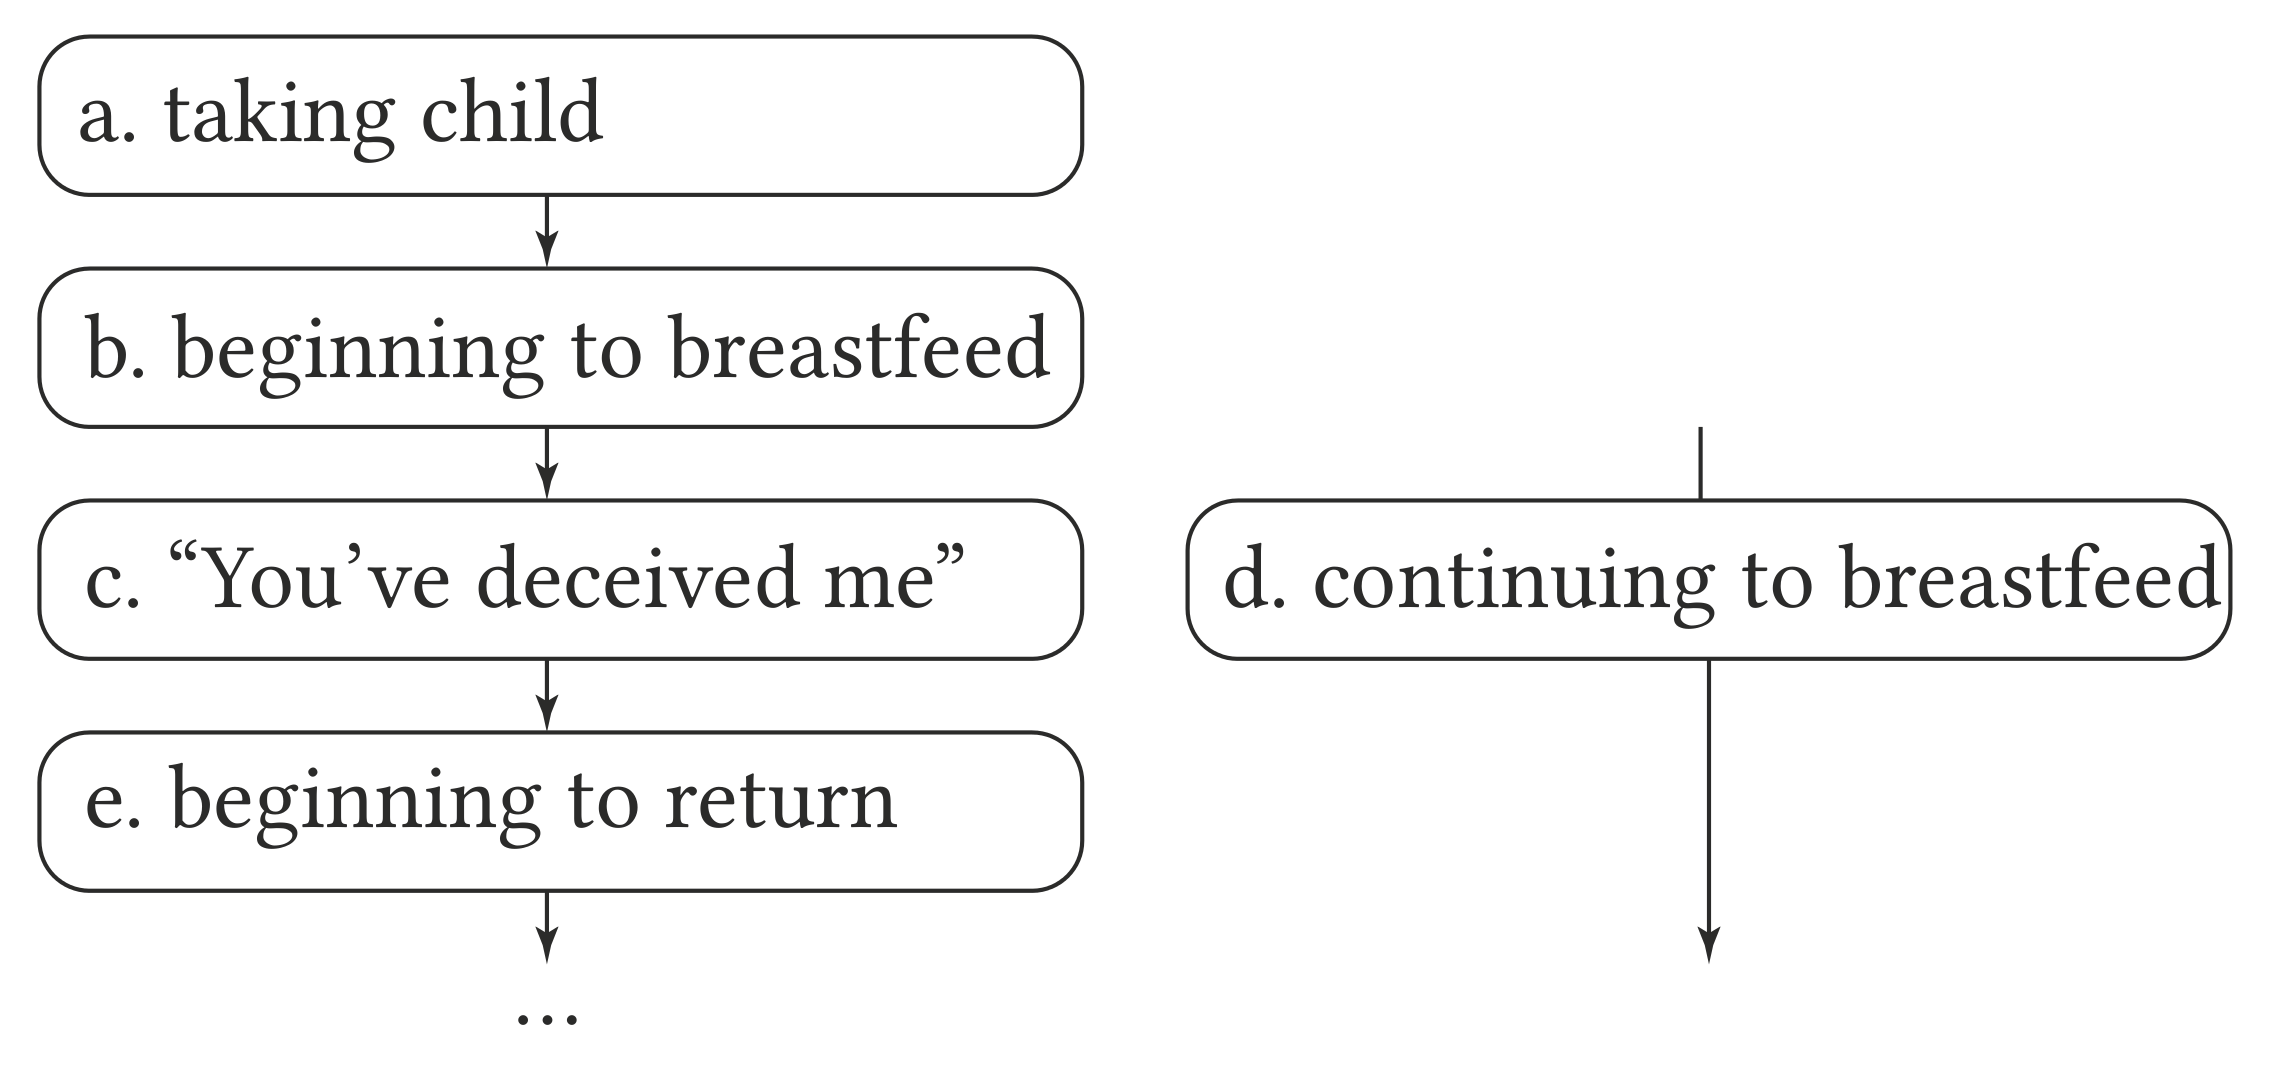
\includegraphics{figures/GrafikRelativeOrderThrowAway.png}
\caption{Relative event order of  (\ref{exNarrProg2})}
\label{FigureRelativeOrderProgressives1}
\end{center}
\end{figure}

\begin{exe}
\ex\label{exNarrProg2}
\begin{xlist}
\ex\label{exNarrProg2Sentence1}\gll a-lɪnkʊ-mmw-eg-a ʊ-mw-anaake\\
1-\textsc{narr}-1-take-\textsc{fv} \textsc{aug}-1-his\_child\\
\glt \lq She took her child.'
\ex\label{exNarrProg2Sentence2}\gll a-lɪnkw-end-a n=ʊ-kʊ-tɪ fi, ʊ-kw-and-a ʊ-kʊ-mm-ongesya\\
a-\textsc{narr}-walk/travel-\textsc{fv} \textsc{com}=\textsc{aug}-15-say what \textsc{aug}-15-begin-\textsc{fv} \textsc{aug}-15-1-breastfeed-\textsc{fv}\\
\glt \lq She then did what, began to breastfeed it.'
\ex\label{exNarrProg2Sentence3}\gll bo ʊ-kʊ-mm-ongesy-a a-lɪnkʊ-tɪ \lq\lq Haa! keet-a ʊʊ-syob-ile, gwe mw-inangʊ. ʊ-t-ile \lq\lq n-daag-ile ʊ-mw-ana''{}''\\
as 1-\textsc{prs}-1-breastfeed-\textsc{fv} 1-\textsc{narr}-say \textsc{interj} \phantom{\lq\lq}watch-\textsc{fv} \textsc{2sg.1sg}-deceive-\textsc{pfv} \textsc{2sg} 1-my\_companion \textsc{2sg}-say-\textsc{pfv} \textsc{1sg}-throw-\textsc{pfv} \textsc{aug}-1-child\\
\glt \lq As she was breastfeeding it, she [the other woman] said \lq\lq Haa! Look, you've deceived me, my friend. You said \lq\lq I've thrown away the child.''{}''{}'
\ex \label{exNarrProg2Sentence4}\gll po jʊ-la \textbf{a}-\textbf{lɪnkw}-\textbf{endelel}-\textbf{a} ʊ-kʊ-mm-ongesy-a ʊ-mw-ana\\
then 1-\textsc{dist} 1-\textsc{narr}-continue-\textsc{fv} \textsc{aug}-15-1-breastfeed-\textsc{fv} \textsc{aug}-1-child\\
\lq That one continued to breastfeed the child.'
\ex \label{exNarrProg2Sentence5}
\gll jʊ-la a-lɪnkw-and-a ʊ-kʊ-buj-a ʊ-kʊ-bʊʊk-a kʊ-kʊ-n-keet-a ʊ-mw-anaake\\
1-\textsc{dist} 1-\textsc{narr}-begin-\textsc{fv} \textsc{aug}-15-return-\textsc{fv} \textsc{aug}-15-go-\textsc{fv} 17-15-1-look-\textsc{fv} \textsc{aug}-1-child\\
\glt \lq That one began returning, going to look for her child.' [Throw away the child]
\end{xlist}
\end{exe}

\largerpage
Example (\ref{exNarrProg3}) depicts the beginning of a race between Hare and Tugutu, a type of bird. While Tugutu remains at the start (\ref{exNarrProg3Sentence4}), Hare does run (\ref{exNarrProg3Sentence2}, \ref{exNarrProg3Sentence5}). Hare's act of running is construed as an ongoing activity contemporaneous with his acts of speaking (\ref{exNarrProg3Sentence3}) and completing the first mile (\ref{exNarrProg3Sentence6}). \figref{FigureRelativeOrderProgressives2} illustrates this as a flow chart.

\begin{exe}
\ex Context: Hare and Tugutu are running a race.
\label{exNarrProg3}
\begin{xlist}
\ex \label{exNarrProg3Sentence1} \gll a-lɪnkʊ-tɪ \textup{\lq\lq}oko kalʊlʊ! tʊ-bop-ege leelo!\textup{''}\\
1-\textsc{narr}-say \phantom{\lq\lq}\textsc{interj} hare(1) \textsc{1pl}-run-\textsc{ipfv.subj} now/but\\
\glt \lq He [Tugutu] said \lq\lq Here we go, Hare! Let's run now!''

\ex\label{exNarrProg3Sentence2} \gll po kalʊlʊ \textbf{a}-\textbf{lɪnkʊ}-\textbf{bop}-\textbf{a}\\
then hare(1) 1-\textsc{narr}-run-\textsc{fv}\\
\glt \lq Hare ran/was running.'

\ex \label{exNarrProg3Sentence3}\gll a-lɪnkʊ-tɪ \textup{\lq\lq}lɪnga tʊ-bop-ile a-ma-elɪ jɪ-mo n-gʊ-kʊ-koolel-a ʊkutɪ \textup{\lq\lq}bʊle, mwa=n-dugutu, ʊ-li-po?\textup{''} gw-itɪk-e ʊ-tɪ \textup{\lq\lq}ee, n-di=po\textup{''{}''}\\
1-\textsc{narr}-say \phantom{\lq\lq}if/when \textsc{1pl}-run-\textsc{pfv} \textsc{aug}-6-mile(<EN) 9-one \textsc{1sg}-\textsc{prs}-\textsc{2sg}-call-\textsc{fv} \textsc{comp} \phantom{\lq\lq}\textsc{q} matronym=9-type\_of\_bird \textsc{2sg}-\textsc{cop}=16 \textsc{2sg}-agree-\textsc{subj} \textsc{2sg}-say.\textsc{subj} \phantom{\lq\lq}yes \textsc{1sg}-\textsc{cop}=16\\
\glt \lq He said \lq\lq When we've run one mile, I'll call you saying \lq\lq Mr. Tugutu are you there?'' You shall answer \lq\lq Yes, I'm here.''{}''{}'\footnote{The narrator oscillates between placing the loanword for \lq mile' in noun class 6, thus re-analyzing /ma/ as a prefix, and placing it in noun class 9a, the default for loans.}

\ex \label{exNarrProg3Sentence4} \gll po bo b-and-ile ʊ-kʊ-bop-a jʊ-la mwa=n-dugutu a-a-syeele pala$\sim$pa-la\\
then as 2-begin-\textsc{pfv} \textsc{aug}-15-run-\textsc{fv} 1-\textsc{dist} matronym=9-t.o.bird 1-\textsc{pst}-remain.\textsc{pfv} \textsc{redupl}$\sim$16-\textsc{dist}\\
\glt  ‎\lq When they had started to run that Mr. Tugutu had remained right there.'

\ex\label{exNarrProg3Sentence5}\gll po kalʊlʊ \textbf{a}-\textbf{lɪnkʊ}-\textbf{bop}-\textbf{a} mw-ene\\
then hare(1) 1-\textsc{narr}-run-\textsc{fv} 1-only\\
\glt \lq So Hare ran/was running alone.'

\ex \label{exNarrProg3Sentence6} \gll a-lɪnkʊ-mal-a a-ma-elɪ ga-mo\\
1-\textsc{narr}-finish-\textsc{fv} \textsc{aug}-6-mile 6-one\\
\glt \lq He completed one mile.' [Hare and Tugutu]
\end{xlist}
\end{exe}

\begin{figure}[hbt]
	\begin{center}
% 		\includegraphics{figures/GrafikRelativeOrderHareTugutu.eps}
		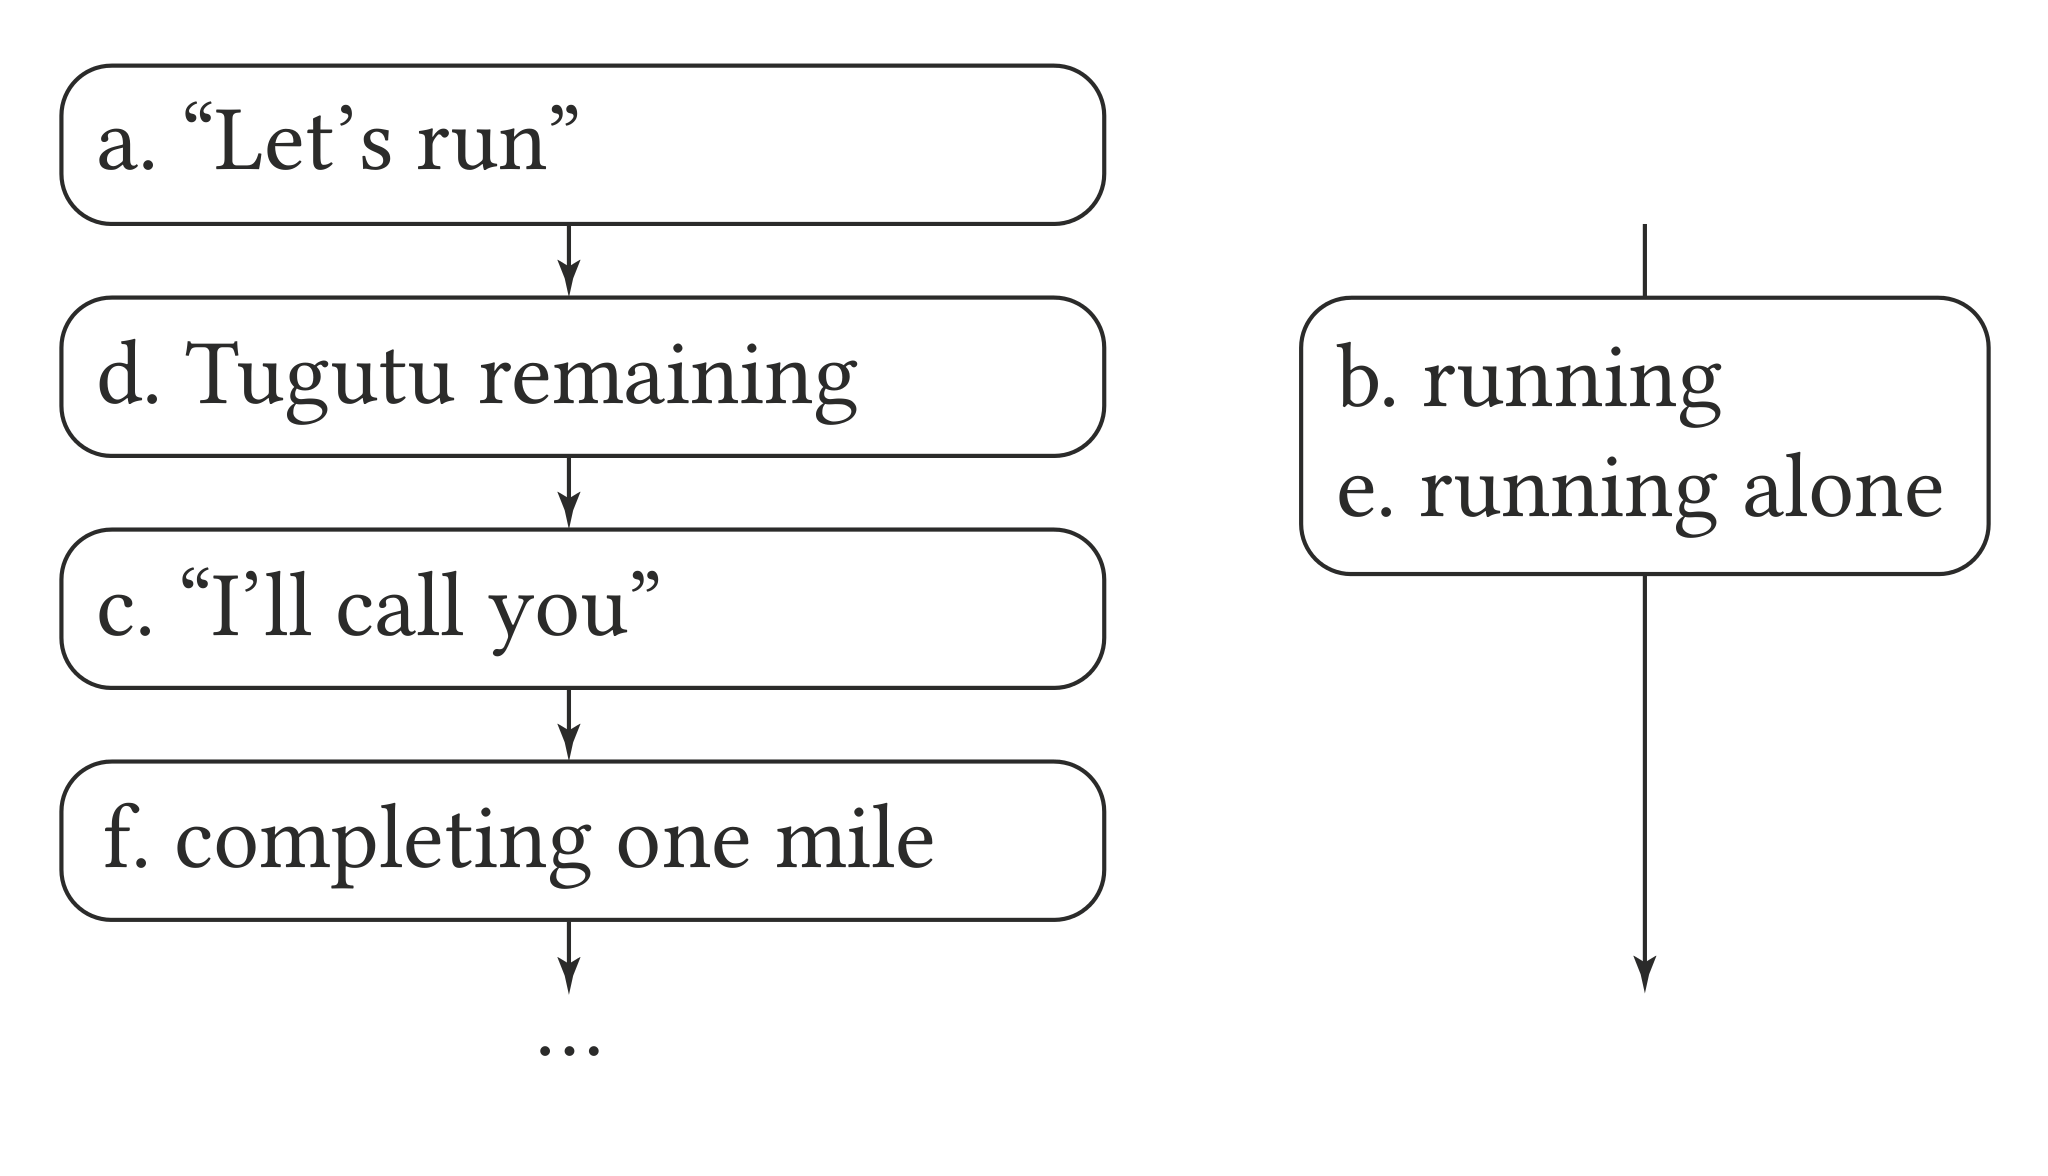
\includegraphics{figures/GrafikRelativeOrderHareTugutu.png}
		\caption{Relative event order of (\ref{exNarrProg3})}
		\label{FigureRelativeOrderProgressives2}
	\end{center}
\end{figure}

To summarize, the semantics of the Nyakyusa narrative tense include past time reference. Further, it is closely linked to episodic events and unspecified for grammatical aspect.

Considering that historically the narrative tense constituted a present tense\is{tense!present} construction, likely one carrying imperfective aspect,\is{aspect!imperfective} this indicates that its employment as a \isi{narrative present} has led to a profound re-adjustment of its semantics. For discussion see \citet{PersohnB2016}, where this shift in meaning is attributed to \citeauthor{FleischmanS1990}'s (\citeyear{FleischmanS1990}) \lq\lq plus interpretation'', by which a \isi{simple present} as the least specific TMA construction takes over the temporal (i.e. past tense)\is{tense!past} and aspectual\is{aspect!grammatical} meaning appropriate to context, as well as to a cross-Bantu tendency to have aspectually underspecified forms as narrative markers. \citet{RobarE2014} convincingly argues that the so-called \textit{wayyiqtol}-construction in \ili{Biblical Hebrew} underwent a comparable change, starting out as a \isi{simple present} whose extensive use as a \isi{narrative present} with the pragmatic function of signalling continuity has led to a bleaching of its original semantic content. In the case of Biblical Hebrew this has gone even further, allowing for the construction in question to take over any kind of tense,\is{tense} aspect\is{aspect!grammatical} or mood.\is{mood}
\is{aspect!grammatical|)}
\subsection{Sequentiality of events}
\label{NARRsequentiality}
Closely linked to the question of aspectual semantics\is{aspect!grammatical} is that of sequential ordering. At first the very concept of a narrative marker may suggest that the Nyakyusa narrative tense denotes sequential ordering of events. Moreover, on the basis of a \ili{Swahili} example taken as typical for Bantu, \citet[121]{NurseD2008} generalizes that ``the narrative explicitly sequences events [\ldots] and says that [\ldots] the second situation is later than the first''. \citet[111]{CoverR2010} cautions againt prematurely accepting such an assumption and observes that sequentiality is not part of the semantics of the narrative paradigms in \ili{Badiaranke} (Northern Atlantic). Similar observations have been made for the \textit{narrative}/\textit{consecutive tense} in the Senufo language \ili{Supyire} \citep{CarlsonR1994} and the so-called \textit{wayyiqtol}-construction in \ili{Biblical Hebrew} \citep{CookJ2004}. Concerning Bantu, \citet[277]{MorrisonME2011}, in her grammar of \ili{Bena} G63, notes that ``[the narrative tense] is \textit{often} best translated as \lq and then X' [emphasis added]'', while \citet{SeidelF2015} makes a similar observation for \ili{Yeyi} R41. Even for Nurse's model example, Swahili,\il{Swahili} a detailed examination shows that not all instances of the paradigm in question feature sequential ordering \citep[112f]{ContiniMoravaE1987}.

\citeauthor{LabovWWaletzkyJ1967}'s (\citeyear{LabovWWaletzkyJ1967}) framework of narrative analysis -- see \sectref{ToolsNarrativeAnalysis} -- provides us with a valuable tool to check whether the Nyakyusa narrative tense inherently encodes sequentiality. Assuming that it does encode an ordering of events would predict that no clause containing it can be displaced without changing the underlying order of events. That is, the narrative tense should only figure in those clauses that are classified as \textit{narrative clauses}.\is{clause types (Labov \& Waletzky)!narrative clause} The discussion of its aspectual semantics, however, has already shown that the narrative tense can have a progressive reading.\is{aspect!progressive} As a function of being ongoing, the eventualities in question overlap with other eventualities. That is, they can be displaced throughout a determined part of the text without changing the underlying order of events and can therefore be classified as \textit{restricted clauses}.\is{clause types (Labov \& Waletzky)!restricted clause} A few additional examples will illustrate the Nyakyusa narrative tense outside of narrative clauses.\is{clause types (Labov \& Waletzky)!narrative clause}

Another representative example of the narrative tense appearing in a restricted clause\is{clause types (Labov \& Waletzky)!restricted clause} is given in (\ref{exNARRnosequence1}). (\ref{exNARRnosequence1sentence1}) contains a husband's orders to his wife and (\ref{exNARRnosequence1sentence2}, \ref{exNARRnosequence1sentence3}) her carrying out these orders. Each step is dependent on the previous one. That is, these three clauses describe eventualities that happen in sequential order. The eventuality described in (\ref{exNARRnosequence1sentence4}), however, takes place simultaneously to the ones described in (\ref{exNARRnosequence1sentence2}, \ref{exNARRnosequence1sentence3}). This means that (\ref{exNARRnosequence1sentence4}) could be anticipated without changing the relative order of events, and is hence a restricted clause.\is{clause types (Labov \& Waletzky)!restricted clause} This becomes clear from the wider context of the story -- he goes on to clandestinely kill her father -- and is also signaled by spatial deixis: his actions take place at the deictic centre (\textit{kʊno} \lq here') while hers is viewed against the ground of an associated \isi{motion} event (see \sectref{jaAspectualizer} on the movement gram (\textit{j})\textit{a}). \figref{FigureRelativeOrderInLaw} is a visualization of the relative order of events.


\begin{exe}
\ex \label{exNARRnosequence1}
\begin{xlist}
\ex \label{exNARRnosequence1sentence1} \gll a-lɪnkʊ-n-koolel-a ʊ-n-kasi, a-lɪnkʊ-tɪ \textup{\lq\lq}n-kasi gw-angʊ, bʊʊk-e lɪlɪno ʊlʊ, k-ʊʊl-e ɪ-fi-lombe, ʊ-ka-sy-e ʊ-bʊ-fu, kʊ-ma-lʊʊka\textup{''}\\
1-\textsc{narr}-1-call-\textsc{fv} \textsc{aug}-1-wife 1-\textsc{narr}-say \phantom{\lq\lq}1-wife 1-\textsc{poss.1sg}, go-\textsc{subj} now/today now \textsc{itv}-buy-\textsc{subj} \textsc{aug}-8-maize \textsc{2sg}-\textsc{itv}-grind-\textsc{subj} \textsc{aug}-14-flour 17-6-store\\
\glt `He called his wife and said ``My wife, go right now, go buy maize, go grind flour, in the stores.''{}'

\ex \label{exNARRnosequence1sentence2} \gll nalooli ʊ-n-kiikʊlʊ \textbf{a}-\textbf{lɪnkw}-\textbf{a} \textbf{k}-\textbf{ʊʊl}-\textbf{a} ɪ-fi-lombe\\
really \textsc{aug}-1-woman 1-\textsc{narr}-go.\textsc{fv} 15-buy-\textsc{fv} \textsc{aug}-8-maize\\
\glt `She went and bought maize.'
\ex \label{exNARRnosequence1sentence3} \gll \textbf{a}-\textbf{lɪnkw}-\textbf{a} \textbf{kʊ}-\textbf{sy}-\textbf{a} ʊ-bʊ-fu kʊ-ma-lʊʊka\\
1-\textsc{narr}-go.\textsc{fv} 15-grind-\textsc{fv} \textsc{aug}-14-flour 17-6-shop\\
\glt `She went and ground flour at the stores.'
\ex \label{exNARRnosequence1sentence4} \gll kʊ-no ʊ-n̩-dʊme \textbf{a}-\textbf{lɪnkʊ}-\textbf{tendekesy}-\textbf{a} ʊ-tʊ-ndʊ, ɪ-fi-lwɪlo fy-a kʊ-n̩-gog-el-a ʊ-gwise\\
17-\textsc{prox} \textsc{aug}-1-husband 1-\textsc{narr}-prepare-\textsc{fv} \textsc{aug}-13-thing \textsc{aug}-8-poison 8-\textsc{assoc} 15-1-kill-\textsc{appl}-\textsc{fv} \textsc{aug}-his\_father(1)\\
\glt `Here her husband prepared things, poison to kill her father with.'
\ex \label{exNARRnosequence1sentence5} \gll a-a-gomok-a ʊ-mw-anike jʊ-la\\
1-\textsc{subsec}-return-\textsc{fv} \textsc{aug}-1-young\_person 1-\textsc{dist}\\
\glt `Then that young woman returned.' [Man and his in-law]
\end{xlist}
\end{exe}

\begin{figure}[hbt]
	\begin{center}
% 		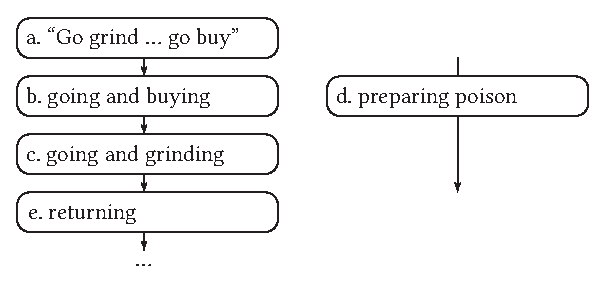
\includegraphics{figures/GrafikRelativeOrderInLaw.eps}
		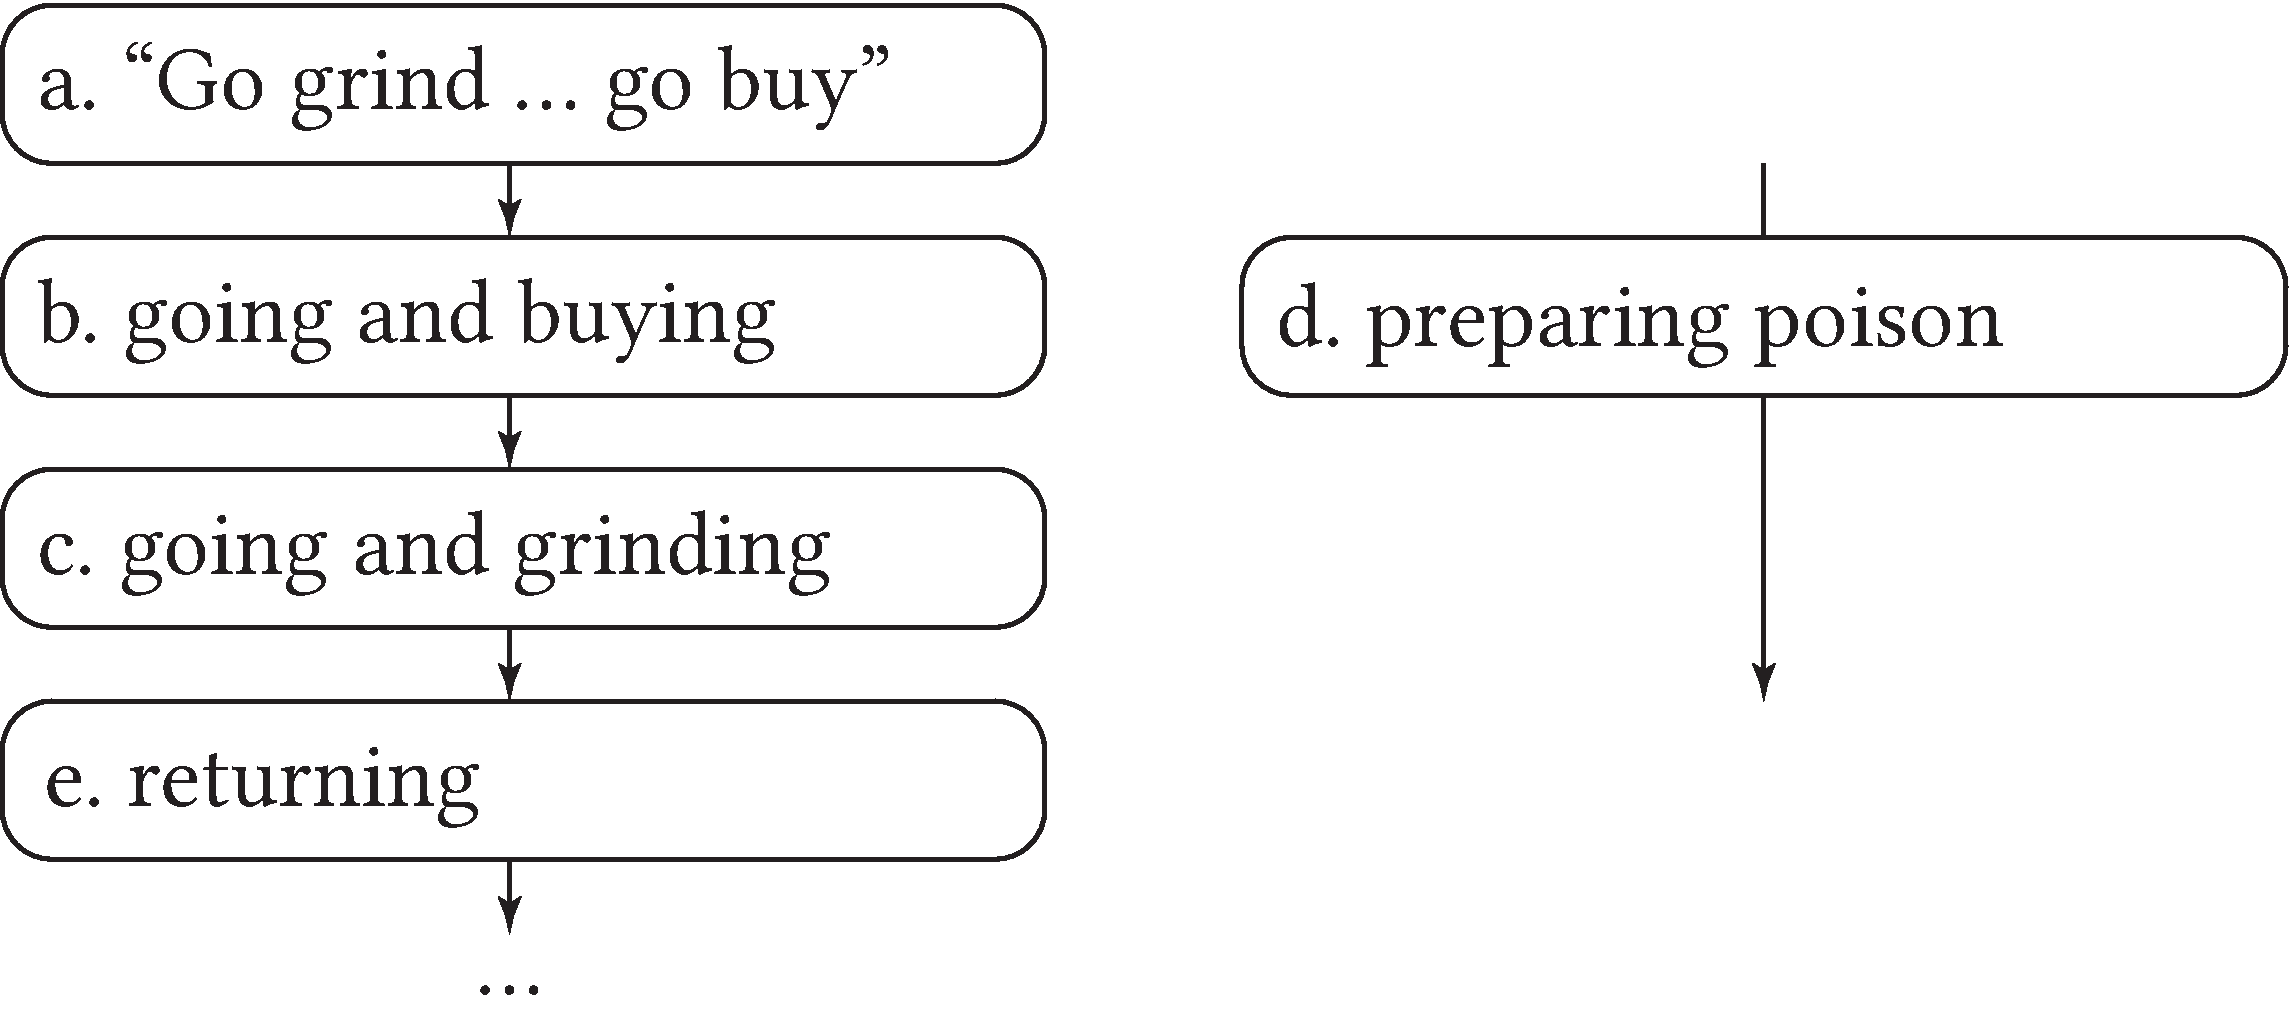
\includegraphics{figures/GrafikRelativeOrderInLaw.png}
	\end{center}
	\caption{Relative event order of (\ref{exNARRnosequence1})}
	\label{FigureRelativeOrderInLaw}
\end{figure}

The narrative tense also features in iconic repetitions that express a single extended eventuality (\ref{exNarrIconicRepetitions}). What is depicted in the three clauses in (\ref{exNarrIconicRepetitionsSentences1}) is not internally ordered. These clauses are thus classified as \textit{co-ordinate clauses}.\is{clause types (Labov \& Waletzky)!co-ordinate clause} The case of (\ref{exNarrIconicRepetitionsSentence2}) presents more difficulties: it is not entirely clear if the speech act depicted takes place during the protagonists' walking or if it is preceded by a stop.

\begin{exe}
\ex \label{exNarrIconicRepetitions}
\begin{xlist}
\ex \label{exNarrIconicRepetitionsSentences1} \gll po \textbf{ba}-\textbf{lɪnkw}-\textbf{end}-\textbf{a}, \textbf{ba}-\textbf{lɪnkw}-\textbf{end}-\textbf{a}, \textbf{ba}-\textbf{lɪnkw}-\textbf{end}-\textbf{a}\\
then 2-\textsc{narr}-walk/travel-\textsc{fv} 2-\textsc{narr}-walk/travel-\textsc{fv} 2-\textsc{narr}-walk/travel-\textsc{fv}\\
\glt \lq They walked, they walked, they walked.'
\ex \label{exNarrIconicRepetitionsSentence2} \gll ba-lɪnkʊ-tɪ \textup{\lq\lq}eh tʊ-kateele\textup{''}\\
2-\textsc{narr}-say \phantom{\lq\lq}\textsc{interj} \textsc{2pl}-be(come)\_tired.\textsc{pfv}\\
\glt \lq They said \lq\lq Eh, we're tired.''{}' [Throw away the child]
\end{xlist}
\end{exe}

Another case of the narrative tense featuring in co-ordinate clauses\is{clause types (Labov \& Waletzky)!co-ordinate clause} is given in
(\ref{exNARRnosequence2}). Clauses (\ref{exNARRnosequence2sentence1}, \ref{exNARRnosequence2sentence2}) describe eventualities that happen in sequence: the pepper only comes out of the bottles after the monkeys catch them. Clauses (\ref{exNARRnosequence2sentence3}--\ref{exNARRnosequence2sentence5}) however, describe various facets of one and the same eventuality. They can be freely swapped with each other, but are ordered relative to (\ref{exNARRnosequence2sentence2}).

\begin{exe}
\ex \label{exNARRnosequence2}
Context: People try to get rid of a group of thieving monkeys that devastate their fields. To fight them, they throw small bottles filled with pepper.
\begin{xlist}
\ex \label{exNARRnosequence2sentence1} \gll si-lɪnkw-angɪl-a m-mwanya\\
10-\textsc{narr}-catch-\textsc{fv} 18-high\\
\glt `They caught (the bottles) in mid air.'

\ex \label{exNARRnosequence2sentence2} \gll ɪ-m-bilipili jɪ-lɪnkʊ-sunyunduk-a n-tʊ-supa mu-la n=ʊ-kʊ-nyeel-el-a m-maa-so na m-mi-lomo \\
\textsc{aug}-9-pepper(<SWA) 9-\textsc{narr}-come\_out\_of-\textsc{fv} 18-13-bottle 18-\textsc{dist} \textsc{com}=\textsc{aug}-15-jump-\textsc{appl}-\textsc{fv} 18-6-eye \textsc{com} 18-4-lip\\
\glt `The pepper came out of the little bottles and flew into their eyes and mouths.'

\ex \label{exNARRnosequence2sentence3} \gll popaa$\sim$po ɪ-n-gambɪlɪ \textbf{si}-\textbf{lɪnkʊ}-\textbf{gw}-\textbf{a} paa-si paapo j-aa-lɪ n-galɪ fiijo\\
\textsc{redupl}$\sim$then \textsc{aug}-10-monkey 10-\textsc{narr}-fall-\textsc{fv} 16-below because 9-\textsc{pst}-\textsc{cop} 9-fierce \textsc{intens}\\
\glt `And so the monkeys fell down because it was very hot.'

\ex \label{exNARRnosequence2sentence4} \gll \textbf{si}-\textbf{lɪnkʊ}-\textbf{kuut}-\textbf{a} si-lɪnkʊ-tɪ, ``Ho! Ho! Ho!''\\
10-\textsc{narr}-cry-\textsc{fv} 10-\textsc{narr}-say \phantom{\lq\lq}\textsc{interj} \textsc{interj} \textsc{interj}\\
\glt `‎‎They cried and said, ``Ho! Ho! Ho!''{}'
\ex \label{exNARRnosequence2sentence5} \gll si-mo \textbf{si}-\textbf{lɪnkʊ}-\textbf{gw}-\textbf{a} paa-si, \textup{\lq\lq}puu!\textup{''}\\
10-one 10-\textsc{narr}-fall-\textsc{fv} 16-below \phantom{\lq\lq}of\_falling\_down\\
\glt `Some fell down, ``Splat!''{}' [Thieving monkeys]
\end{xlist}
\end{exe} %d.h. einen restricted clause

To conclude, the Nyakyusa narrative tense appears in narrative clauses\is{clause types (Labov \& Waletzky)!narrative clause} as well as in restricted\is{clause types (Labov \& Waletzky)!restricted clause} and co-ordinate clauses.\is{clause types (Labov \& Waletzky)!co-ordinate clause} This shows that sequential order is not one of its semantic features. The fact that most eventualities depicted in this paradigm stand in sequence is a mere correlate of the predominantly iconic ordering of narrative discourse.

However, it is important to note that while in examples (\ref{exNarrProg2}--\ref{exNARRnosequence2}) not all the eventualities depicted in the narrative tense are ordered relative to each other, no out-of-sequence uses are attested. The narrative tense does not feature in free clauses.\is{clause types (Labov \& Waletzky)!free clause}  Although it does feature in certain restricted clauses,\is{clause types (Labov \& Waletzky)!restricted clause} this is limited to clearly defined episodic situations; see also \sectref{NARRpast}. That is, the narrative tense does not feature in clauses that serve as orientation; see also \sectref{NarrativeMarkersUseDistribution}. Lastly, flashbacks in narrative discourse are exclusively expressed by means of the past perfective (\sectref{PastPFVNarrativeDiscourseSupportive}).
\subsection{Summary}
To summarize, the Nyakyusa narrative tense goes back to a \isi{simple present} or present progressive\is{aspect!progressive} used as a narrative present.\is{narrative present} In the present-day language, it is the most common dedicated narrative marker (see \sectref{NarrativeMarkersQuantitativeDistribution}), whose semantics include reference to the past time. It is unspecified for grammatical aspect,\is{aspect!grammatical} but restricted to episodic situations and thus the narrative storyline. The narrative tense by itself does not encode sequential ordering. Instead it is attested with sequential as well as simultaneous eventualities. The employment of the narrative tense, like the subsecutive,\is{subsecutive} is dependent on an otherwise established situation and forms part of a larger pattern, in which narrative discourse is constructed around the notion of \isi{thematic continuity} and discontinuity.  Given that the narrative tense is a dedicated marker of narrative  discourse, the narrative tense can further be understood as a metalinguistic\is{component of meaning!metalinguistic} signal of narrativity.
\is{narrative tense|)}
\section{Subsecutive}\label{Subsecutive}\is{subsecutive|(}
This section deals with the subsecutive, Nyakyusa's second dedicated narrative marker. In the following sub-sections, first its formal makeup and possible diachronic source will be discussed (\sectref{SubsecutiveIntroduction}), then some restrictions on the use of the subsecutive will be broached (\sectref{SubsecutiveAndNarrative}). This is followed by an overview of its semantics together with its basic textual function\is{component of meaning!textual} (\sectref{SubsecutiveSemantics}), as these two facets are inseparably linked. The latter are then illustrated by a number of common uses (\sectref{SubsecutiveCommon}) before going on to discuss a number of examples of the subsecutive without strict temporal progression (\sectref{SubsecutiveCounterExamples}).
\subsection{Formal makeup}\label{SubsecutiveIntroduction}
\largerpage
The subsecutive is formed by a prefix \textit{a}- in the post-initial slot, together with the default final vowel -\textit{a}.

\begin{exe}
\ex \textit{twajoba} `then we spoke'
\end{exe}

There is no \isi{negative} counterpart to the subsecutive. In elicitation, negation of the subsecutive through the \isi{negative} \isi{auxiliary} \textit{sita} plus an augmentless infinitive,\is{infinitive} parallel to what is found for the \isi{narrative tense} (see \sectref{sectionNarrativeTenseFormalAspects}), was accepted. This pattern is, however, not attested in the text corpus. Like the narrative tense,\is{narrative tense} the subsecutive is attested only in independent clauses.

\citet{SchumannK1899} and \citet{EndemannC1914} consider the subsecutive a simple past,\is{tense!past}\footnote{They refer to it as \textit{Imperfektum}. In the German tradition this term is sometimes used as a synonym for \textit{Präteritum} (preterite/simple past\is{tense!past}), which fits their description.} an analysis that is, however, not corroborated by its usage in text collections from the chronolect described by them (\citealt{BergerP1933}; \citealt{BusseJ1942}; \citeyear{BusseJ1949}). The term \textit{subsecutive} has been adopted from \citeauthor{MwangokaNVoorhoeveJ1960b}'s (\citeyear{MwangokaNVoorhoeveJ1960b}) grammatical sketch. Some of the uses of this construction found in \citeauthor{MeyerT1989}'s (\citeyear{MeyerT1989}) ethnological notes, originally gathered at the turn of the twentieth century, indicate that the subsecutive constitutes a former present perfective\is{tense!present}\is{aspect!perfective} or anterior.\is{aspect!anterior} Such an origin is also indicated by the \isi{evidential} of report \textit{baatɪ} (\sectref{defectiveti}), most likely from \lq they (have) said', and the two variants of the courtesy formula \textit{naapela} / \textit{mbelile} `please', the former featuring the subsecutive, the latter the present perfective.\is{tense!present}\is{aspect!perfective} What is more, as the following discussion will show, a diachronic source along the lines of a present perfective\is{tense!present}\is{aspect!perfective} or anterior\is{aspect!anterior} is consistent with the meaning and use of the subsecutive in the present day language.

\subsection{Restrictions on use}\label{SubsecutiveAndNarrative}
As discussed in \sectref{NarrativeMarkersQuantitativeDistribution}, the subsecutive is the less frequent of Nyakyusa's two narrative markers, considering the absolute frequency within a given text as well as across the entire corpus of oral narratives. Unlike the narrative tense,\is{narrative tense} which no narrative in the corpus can do without, the subsecutive is completely absent from nearly half of all oral narratives. What is more, the subsecutive is subject to normative restrictions.

To begin with, the subsecutive does not appear in written narratives, with the exception of one sole token. In discussions of examples from oral narratives, some of the language assistants stated that the subsecutive is a common device in storytelling, but followed up by saying that it would be inappropriate in the written medium.\footnote{A similar phenomenon has been observed in \ili{Malila} M24, where speakers would use the present perfective,\is{tense!present}\is{aspect!perfective} likewise of the shape \textit{a}-\textsc{vb}-\textit{a}, in the storyline of oral narratives, but insisted that it would be inappropriate for a written story \citep[24]{EatonH2015a}.} Other language assistants rejected any constructed examples containing the subsecutive but then used it themselves in oral texts. A few speakers even considered this construction a \ili{Ndali} intrusion into their language. This assessment can easily be rejected, given the construction's apparent age, the fact that it is found in the eastern varieties of Nyakyusa (\sectref{InternalClassiffication}), whereas \ili{Ndali} is one of Nyakyusa's western neighbours, and its distribution, which does not resemble that of its \ili{Ndali} cognate as described by \citet{BotneR2008}.

\largerpage
\subsection{Semantics and basic textual function}\label{SubsecutiveSemantics}
As discussed in \sectref{NARRpast}, narrative markers across languages differ, among other ways, in their possible temporal reference. The Nyakyusa subsecutive, like the narrative tense,\is{narrative tense} is attested only with temporal reference preceding the time of speech. This is corroborated by negative evidence from elicitation, where it was rejected for future\is{tense!future} predictions (\ref{exSubsecNotFuture1}, \ref{exSubsecNotFuture2}) as well as in a timeless \isi{generic} use (\ref{exSubsecNotGeneric}).
\begin{exe}


\newpage 
\ex \label{exSubsecNotFuture1} Context: A young man's plans for the future.
\begin{xlist}
\ex[]{\gll bo n-gʊl-ile a=n-gʊ-jeng-a ɪɪ-nyumba ɪɪ-nywamu\\
as \textsc{1sg}-grow-\textsc{pfv} \textsc{fut}=\textsc{1sg}-\textsc{prs}-build-\textsc{fv} \textsc{aug}-house(9) \textsc{aug}-big(9)\\}
\ex[\#]{\gll \textbf{n}-\textbf{aa}-\textbf{tim}-\textbf{a} ɪɪ-ng'ombe pa-ka-aja\\
\textsc{1sg}-\textsc{subsec}-herd-\textsc{fv} \textsc{aug}-cow(10) 16-12-homestead\\
\glt (intended: \lq When I am grown up, I will build a big house. Then I will herd cows at home.')}
\end{xlist}
\ex \label{exSubsecNotFuture2} Context: Talking about the speaker's plans for tomorrow.
\begin{xlist}
\ex[]{\gll kɪ-laabo a=n-gʊ-kin-a ʊ-m-pɪla\\
7-tomorrow \textsc{fut}-\textsc{1sg}-\textsc{prs}-play-\textsc{fv} \textsc{aug}-3-ball\\}
\ex[\#]{\gll bo m-mal-ile pa-kʊ-kin-a \textbf{n}-\textbf{aa}-\textbf{bʊʊk}-\textbf{a} kʊ-n-nuguna gw-angʊ kʊ-kʊ-ly-a nagwe ɪ-fi-ndʊ fy-a pa-muu-si\\
as \textsc{1sg}-finish-\textsc{pfv} 16-15-play-\textsc{fv} \textsc{1sg}-\textsc{subsec}-go-\textsc{fv} 17-1-younger\_sibling\_of\_same\_sex 1-\textsc{poss.1sg} 17-15-eat-\textsc{fv} \textsc{com.1} \textsc{aug}-8-food 8-\textsc{assoc} 17-3-daytime\\
\glt (intended: \lq Tomorrow I will play football. When I am done playing, I will go to my younger brother to have lunch with him.')}
\end{xlist}
\ex \label{exSubsecNotGeneric} Context: Describing the process of preparing stiff porridge.
\begin{xlist}
\ex[]{\gll bi-kʊ-kosy-a ʊ-m-ooto\\
2-\textsc{prs}-light-\textsc{fv} \textsc{aug}-3-fire\\}
\ex[\#]{\gll \textbf{b}-\textbf{aa}-\textbf{suk}-\textbf{a} ɪ-fy-a kʊ-pɪɪj-ɪl-a\\
2-\textsc{subsec}-wash-\textsc{fv} \textsc{aug}-8-\textsc{assoc} 15-cook-\textsc{appl}-\textsc{fv}\\}
\ex[\#]{\gll \textbf{b}-\textbf{aa}-\textbf{bɪɪk}-\textbf{a} a-m-ɪɪsi pa-m-ooto \ldots\\
2-\textsc{subsec}-put-\textsc{fv} \textsc{aug}-6-water 16-3-fire\\
\glt (intended: \lq They light the fire. Then they wash the cooking utensils. Then they put the water on the fire \ldots')}
\end{xlist}
\end{exe}

Like the narrative tense,\is{narrative tense} the subsecutive is only attested in episodic sentences, that is reports of specific events or occasions; see \sectref{NARRpast} for discussion. Negative evidence from elicitation shows that even within the past\is{tense!past} it cannot continue habituals\is{aspect!habitual} or generics:\is{aspect!generic}

\begin{exe}
\ex
\begin{xlist}
\ex[]{\gll ijolo ba-a-mog-aga fiijo\\
old\_times 2-\textsc{pst}-dance-\textsc{ipfv} \textsc{intens}\\
}
\ex[]{\gll ba-a-fwal-aga kanunu fiijo\\
2-\textsc{pst}-dress/wear-\textsc{ipfv} well \textsc{intens}\\}
\ex[\#]{\gll b-oog-a\\
2-\textsc{subsec}.bathe-\textsc{fv}\\}
\ex[\#]{\gll ba-a-sanjʊl-a n=ɪɪ-nywili \ldots\\
2-\textsc{subsec}-comb-\textsc{fv} \textsc{com}=\textsc{aug}-hair(10) {}\\
\glt (intended: \lq Long ago they used to dance a lot. They dressed well. They bathed. They combed their hair \ldots')}
\end{xlist}
\end{exe}

Concerning its aspectual semantics,\is{aspect!grammatical} the subsecutive, unlike the narrative tense,\is{narrative tense} always has a perfective reading;\is{aspect!perfective} see \sectref{PerfectivityCompletion} for a discussion of perfectivity. What is more, the subsecutive explicitly marks a step forward in the text. In this it can be understood as a verbal variety of what \citet{DooleyRALevinsohnSH2000} call a \lq\lq developmental marker'', which \lq\lq indicate[s] that the material so marked represents a new development in the story or argument, as far as the author's purpose is concerned'' (p. 48). This function will become clear when looking at its common uses in \sectref{SubsecutiveCommon}. In the majority of cases, the narrative development goes along with an advancement of narrative time. Thus, the subsecutive nearly exclusively occurs in narrative clauses,\is{clause types (Labov \& Waletzky)!narrative clause} i.e. those clauses that stand in fixed sequence; see \sectref{ToolsNarrativeAnalysis} for \citeauthor{LabovWWaletzkyJ1967}'s (\citeyear{LabovWWaletzkyJ1967}) classification of independent clauses within narratives. Unlike the narrative tense,\is{narrative tense} the subsecutive is not attested in restricted clauses.\is{clause types (Labov \& Waletzky)!restricted clause} A few cases of the subsecutive in co-ordinate\is{clause types (Labov \& Waletzky)!co-ordinate clause} clauses will be examined more closely in \sectref{SubsecutiveCounterExamples}. Closely linked to this distribution, the only type of temporal adverbials the subsecutive is attested with is adverbials referring to a subsequent time span. (\ref{exSubsecutiveSerieSentence2}) illustrates the latter for a temporal clause,\is{subordinate clauses!temporal clause} (\ref{exSubsecutiveSerieSentence5}) for the adverbial \textit{kɪlaabo} \lq tomorrow, next day'. 

\begin{exe}
\ex Context: A girl has eloped with a man. Her father has found out where they are.
\begin{xlist}
\ex \label{exSubsecutiveSerieSentence1} \gll po piitaasi ʊ-n-nyambala jʊ-la a-lɪnkʊ-j-a mu-ndʊ gw-a kʊ-fung-a ɪɪ-safalɪ j-aake j-aa kʊ-bʊʊk-a kʊ-no ba-li=ko ba-la, kʊ-kʊ-mel-a ɪ-fy-ʊma\\
then later \textsc{aug}-1-man 1-\textsc{dist} 1-\textsc{narr}-be(come)-\textsc{fv} 1-person 1-\textsc{assoc} 15-tie-\textsc{fv} \textsc{aug}-journey(9)(<SWA) 9-\textsc{poss.sg} 9-\textsc{assoc} 15-go-\textsc{fv} 17-\textsc{prox} 2-\textsc{cop}=17 2-\textsc{dist} 17-15-claim-\textsc{fv} \textsc{aug}-8-rich\\
\glt \lq Then later that man started to set out for where they were, in order to claim the brideprice.'
\ex \label{exSubsecutiveSerieSentence2}\gll \textbf{bo} \textbf{a}-\textbf{fik}-\textbf{ile} kʊ-la \textbf{b}-\textbf{a}-\textbf{mmw}-\textbf{ambɪlɪl}-\textbf{a} kanunu\\
as 1-arrive-\textsc{pfv} 17-\textsc{dist} 2-\textsc{subsec}-1-receive-\textsc{fv} well\\
\glt \lq When he arrived there, they received him well.'

\ex \gll a-a-ly-a\\
1-\textsc{subsec}-eat-\textsc{fv}\\
\glt \lq He ate.'

\ex \gll a-a-gon-a\\
1-\textsc{subsec}-rest-\textsc{fv}\\
\glt \lq He slept.'

\ex \label{exSubsecutiveSerieSentence5} \gll po \textbf{kɪ}-\textbf{laabo} \textbf{a}-\textbf{mmw}-\textbf{eg}-\textbf{a} ʊ-n-kyameni n=ʊ-kʊ-m̩-bʊʊl-a ɪ-si si-n-twele pa-la\\
then 7-tomorrow 1.\textsc{subsec}-1-take-\textsc{fv} \textsc{aug}-1-chairman(<EN) \textsc{com}=\textsc{aug}-15-1-tell-\textsc{fv} \textsc{aug}-\textsc{prox.10} 10-1-carry.\textsc{pfv} 16-\textsc{dist}\\
\glt \lq The next day he contacted  a chairman and told him what brought him there.' [Man and his in-law]

\end{xlist}
\end{exe}

Consecutive clauses featuring the subsecutive are generally understood as depicting an ordered sequence of completed\is{completion} eventualities building on each other, as in (\sectref{exSubsecutiveSerieSentence1}--\ref{exSubsecutiveSerieSentence5}). A few exceptions, in which a sequence of clauses featuring the subsecutive group together, will be examined in \sectref{SubsecutiveCounterExamples}.

Note at this point that the opposition between the \isi{narrative tense} and the subsecutive in the present-day language cannot be reduced merely to one of grammatical aspect. As discussed in \sectref{NARRpast}, the \isi{narrative tense} is best understood as unspecified for aspect and allows for a perfective-like\is{aspect!perfective} reading, too. Rather, these two paradigms form an opposition between the default, all-purpose narrative tense on the one hand and the subsecutive as the more restricted, specifically perfective\is{aspect!perfective} marker of a narrative development on the other.

\subsection{Common occurrences}
\label{SubsecutiveCommon}
Many tokens of the subsecutive in the corpus are found in discernible, reoccurring environments. To begin with, it is found in pairings with the narrative tense,\is{narrative tense} as in (\ref{exSubsecutivePreparationResultSentence2}, \ref{exSubsecutivePreparationResultSentence3}) and (\ref{exSubsecutivePreparationResultSentence5}, \ref{exSubsecutivePreparationResultSentence6}), in which a situation is depicted first in its inception or preparation and then in its culmination.


\begin{exe}
\ex \label{exSubsecutivePreparationResult}
\begin{xlist}
\ex \gll po ba-lɪnkw-and-a b-oope bo bʊ-k-iile n=ʊ-lʊ-bʊnjʊ\\
then 2-\textsc{narr}-begin-\textsc{fv} 2-also as 14-dawn-\textsc{pfv} \textsc{com}=\textsc{aug}-11-morning\\
\glt \lq Early in the morning they started.'

\ex \label{exSubsecutivePreparationResultSentence2}\gll ba-lɪnkʊ-j-a b-andʊ ba-a k-oog-a b-ooga\\
2-\textsc{narr}-be(come)-\textsc{fv} 2-person 2-\textsc{assoc} 15-bathe-\textsc{fv} 14-bath\\
\glt \lq They began to bath.'

\ex \label{exSubsecutivePreparationResultSentence3}\gll \textbf{ba}-\textbf{a}-\textbf{fwal}-\textbf{a} kanunu\\
2-\textsc{subsec}-dress/wear-\textsc{fv} well\\
\glt \lq They got dressed up.'

\ex \label{exSubsecutivePreparationResultSentence4}\gll ba-lɪnkʊ-j-a b-andʊ ba-a kʊ-piny-a ɪ-mi-sigo gy-abo n=ʊ=kʊ-bʊʊk-a\\
2-\textsc{narr}-be(come)-\textsc{fv} 2-person 2-\textsc{assoc} 15-bind-\textsc{fv} \textsc{aug}-4-burden 4-\textsc{poss.pl} \textsc{com}=\textsc{aug}-15-go-\textsc{fv}\\
\glt \lq They began to bind their things and go.'

\ex \label{exSubsecutivePreparationResultSentence5} \gll a-lɪnkʊ-pimb-a ʊ-bʊ-fu bw-ake n̩goosi\\
1-\textsc{narr}-load-\textsc{fv} \textsc{aug}-14-flour 14-\textsc{poss.sg} N.\\
\glt \lq Ngoosi lifted that flour.'

\ex \label{exSubsecutivePreparationResultSentence6} \gll \textbf{ii}-\textbf{twɪk}-\textbf{a} pa-n-tʊ\\
1.\textsc{subsec}.\textsc{refl}-lift\_to\_head-\textsc{fv} 16-3-head\\
\glt \lq She loaded it on her head.' [Man and his in-law]
\end{xlist}
\end{exe}
Interestingly, \citet[ch. 6]{FleischmanS1990} notes a mostly parallel pattern in \ili{Old French} epics, which consists of depicting certain eventualities through an alternation of a \isi{narrative present} followed by the present anterior\is{tense!present}\is{aspect!anterior} (\textit{passé composé} in the francophone tradition). The latter in that early romance variety came close to a present perfective.\is{aspect!perfective} She goes on to observe that

\begin{quote}
the first situation is presented in its inception [\ldots] and the second as completed [\ldots], it is as if the first precipitates the second to its conclusion, uniting the two into a global event [\ldots] Tense switches of this type, which operate to split a macro-event into its constituent phases, are a common device for establishing cohesion. The distinct phases reported by verbs in individual clauses are bound together into complex predicates \citep[196f]{FleischmanS1990}
\end{quote}

Recall from  \sectref{SubsecutiveIntroduction} that there are a number of independent indications that the subsecutive constitutes a former present anterior\is{tense!present}\is{aspect!anterior} or present perfective,\is{aspect!perfective} while the source of the \isi{narrative tense} is doubtless a former imperfective present\is{aspect!imperfective} (\sectref{NarrativePresent}). Pairings such as (\ref{exSubsecutivePreparationResultSentence2}, \ref{exSubsecutivePreparationResultSentence3}) and (\ref{exSubsecutivePreparationResultSentence5}, \ref{exSubsecutivePreparationResultSentence6}) can thus be understood as another case in point and may well be the source of the present-day functions of the subsecutive. 

In a fashion similar to the preceding example, the movement\is{motion} gram (\textit{j})\textit{a} (\sectref{jaAspectualizer}) is commonly found in the subsecutive with \textit{fika} `arrive' as its complement and following iconic repetitions of \textit{enda} `walk, travel' in the \isi{narrative tense} (\ref{exSubsecutiveJaKufikaRepetitionEnda}). This can be understood as closing the macro-event of \isi{motion} on the one hand, while on the other advancing the text by indicating the conclusion of a prolonged journey. Note also how temporal and spatial progression in this case go together in one complex predicate. A variation of this theme is found in (\ref{exSubsecutiveJaKufikaEndelela}), where the subsecutive follows \textit{endelela} `continue (the journey)'.


\begin{exe}
\ex \label{exSubsecutiveJaKufikaRepetitionEnda}
\begin{xlist}
\ex\gll b-oosa ba-bɪlɪ ba-lɪnkʊ-j-a ba-ndʊ ba-a kʊ-bʊʊk-a m̩-bʊ-ganga\\
2-all 2-two 2-\textsc{narr}-be(come)-\textsc{fv} 2-person 2-\textsc{assoc} 15-go-\textsc{fv} 18-1-doctor\\
\glt `The two of them set out to go to a healer.'
\ex\gll boo=bʊno$\sim$bʊ-no ba-lɪnkw-end-a, ba-lɪnkw-end-a, ba-lɪnkw-end-a, ba-lɪnkw-end-a n=ʊ-kw-end-a\\
\textsc{ref.14}=\textsc{redupl}$\sim$14-\textsc{dem} 2-\textsc{narr}-walk/travel-\textsc{fv} 2-\textsc{narr}-walk/travel-\textsc{fv} 2-\textsc{narr}-walk/travel-\textsc{fv} \textsc{com}=\textsc{aug}-15-walk/travel-\textsc{fv} \textsc{com}=\textsc{aug}-15-walk/travel-\textsc{fv}\\
\glt `Thus they travelled, travelled, travelled and travelled.'
\ex\gll \textbf{ba}-\textbf{a}-\textbf{j}-\textbf{a} kʊ-\textbf{fik}-a n-k-iisʊ kɪ-mo\\
2-\textsc{subsec}-go-\textsc{fv} 15-arrive-\textsc{fv} 18-7-land 7-one\\
\glt `Finally they arrived in some land.' [Pregnant women]
\end{xlist}
\ex \label{exSubsecutiveJaKufikaEndelela}
\begin{xlist}
\ex \gll ba-alɪnkw-endelel-a n=ɪɪ-safalɪ\\
2-\textsc{narr}-continue-\textsc{fv} \textsc{com}=\textsc{aug}-journey(9)(<SWA)\\
\glt \lq They continued their journey.'
\ex \gll po balɪnkw-endelel-a bʊbʊʊ$\sim$bʊ\\
then 2-\textsc{narr}-continue-\textsc{fv} \textsc{redupl}$\sim$\textsc{prox.14}\\
\glt \lq Thus they continued.'
\ex\gll \textbf{ba}-\textbf{a}-\textbf{j}-\textbf{a} kʊ-\textbf{fik}-a n-ky-eni kangɪ\\
 2-\textsc{subsec}-go-\textsc{fv} 15-arrive-\textsc{fv} 18-7-forehead again\\
\glt `They got further ahead.' [Man and his in-law]
\end{xlist}
\end{exe}

This use of the subsecutive to conclude a macro-event and at the same time advance the story is also found on a bigger scale. (\ref{exSubsecutiveHareTugutu}) is an abridged version of a narrative episode in which Tugutu, a type of bird, prepares a racetrack in order to outwit Hare. The subsecutive in (\ref{exSubsecutiveHareTugutuSentence6}) concludes the preparation episode and leads over to the next episode, the race itself. See (\ref{exNARRnosequence1}) on p.\nobreakspace\pageref{exNARRnosequence1sentence5} for a comparable example of the subsecutive concluding an extensive macro-event. 

\begin{exe}
\ex \label{exSubsecutiveHareTugutu}
Context: Tugutu (a type of bird) has challenged Hare to a race. He has gathered five companions.
\begin{xlist}

\ex \gll mwa=n-dugutu a-a-bʊʊk-ile\\
matronym=9-type\_of\_bird 1-past-go-\textsc{pfv}\\
\glt \lq Mr. Tugutu went.'

\ex \gll a-a-ba-paal-ile a-ba-nine ba-haano \ldots\\
1-\textsc{pst}-2-invite-\textsc{pfv} \textsc{aug}-2-companion 2-five {}\\
\glt \lq He gathered five companions \ldots'


\ex \label{exSubsecutiveHareTugutuSentence3} \gll bo ii-sikʊ ly-a kɪ-laabo, bo lɪ-fik-ile, mwa=n-dugutu a-alɪ-m̩-bɪɪk-ile mwa=n-dugutu n-nine pa-bw-andɪlo\\
as 5-day 5-\textsc{assoc} 7-tomorrow as 5-arrive-\textsc{pfv} matronym=9-t.o.bird 1-\textsc{pst}-1-put-\textsc{pfv} matronym=9-t.o.bird 1-companion 16-14-start\\
\glt \lq When the next day arrived, Mr. Tugutu placed a fellow Mr. Tugutu at the start.'

\ex \label{exSubsecutiveHareTugutuSentence4} \gll kangɪ maelɪ jɪ-ngɪ jɪ-mo a-alɪ-m̩-bɪɪk-ile mwa=n-dugutu n-nine \ldots\\
again mile(9)(<EN) 9-other 9-one 1-\textsc{pst}-1-put-\textsc{pfv} matronym=9-t.o.bird 1-companion {}\\
\glt \lq Another mile, he placed a fellow Mr. Tugutu \ldots'

\ex \label{exSubsecutiveHareTugutuSentence5} \gll na kʊ-lʊ-malɪɪkɪlo, ma-elɪ ga-a bʊ-haano mwa=n-dugutu ʊ-jʊ-ngɪ\\
\textsc{com} 17-11-end 6-mile 6-\textsc{assoc} 5-five matronym=9-t.o.bird \textsc{aug}-1-other\\
\glt \lq At the finish line, the fifth mile, another Mr. Tugutu.'

\ex \label{exSubsecutiveHareTugutuSentence6} \gll po mwa=n-dugutu ʊ-jʊ-ngɪ, jʊ-la ba-a-job-aga na kalʊlʊ \textbf{a}-\textbf{a}-\textbf{j}-\textbf{a} pa-bw-andɪlo pa-la\\
then matronym=9-t.o.bird \textsc{aug}-1-other 1-\textsc{dist} 2-\textsc{pst}-speak-\textsc{ipfv} \textsc{com} hare(1) 1-\textsc{subsec}-be(come)-\textsc{fv} 16-14-start 16-\textsc{dist}\\
\glt \lq  ‎‎The other Mr. Tugutu, the one who had been talking with Hare, he then was at the start.' [Hare and Tugutu]
\end{xlist}
\end{exe}%FN wegen mile und ncl 9a/6 kopieren?

Interestingly, \citet[143ff]{CraneTM2011} observes that, in \ili{Totela} K41, a hodiernal perfective\is{aspect!perfective} -- she speaks of a marker of \lq\lq nuclear completion'';\is{completion} see \sectref{PerfectivityCompletion} for discussion -- is similarly employed at the boundary of scenes or episodes within narratives, where it marks the \lq\lq completion of one set of activities and the commencement of another''. The situation in that particular language, however, differs from Nyakyusa in that the verbal paradigm in question is fully operative outside of narrative discourse.

Another recurring device in the narrative corpus consists of a past imperfective\is{tense!past}\is{aspect!imperfective} verb followed by one in the subsecutive. In these pairs, the imperfective\is{aspect!imperfective} depicts a setting, while the subsecutive verb constitutes a progression that evolves out of, and ruptures, the preceding situation. (\ref{exSubsecPigDuck}) gives the opening four sentences of a short narrative. (\ref{exSubsecPigDuckSentence1}) constitutes the orientation section,\is{section!orientation} while (\ref{exSubsecPigDuckSentence2}) sets the stage for the upcoming event. Duck's pecking for food is a continuous activity and accordingly it is depicted in the past imperfective.\is{tense!past}\is{aspect!imperfective} With (\ref{exSubsecPigDuckSentence3}), the complicating action\is{section!complicating action} of the narrative begins. Duck's search ends with the sight of Pig's food, which is marked by use of the subsecutive plus \textit{enda} `walk/travel' as an ingressive auxiliary.\is{auxiliary} This sets the ball rolling and leads to the ultimately fatal act described in (\ref{exSubsecPigDuckSentence4}).

\begin{exe}
\ex \label{exSubsecPigDuck}
\begin{xlist}
\ex \label{exSubsecPigDuckSentence1}\gll ɪ-li-sikʊ lɪ-mo, ɪ-n-gʊlʊbe j-aa-bɪɪk-ɪl-iigwe ɪ-fi-ndʊ fy-ake\\
\textsc{aug}-5-day 5-one \textsc{aug}-9-pig 9-\textsc{pst}-put-\textsc{appl}-\textsc{pass.pfv} \textsc{aug}-8-food 8-\textsc{poss.sg}\\
\glt `One day, Pig was given its food.'

\ex\label{exSubsecPigDuckSentence2}\gll po leelo ɪ-li-seekwa \textbf{ly}-\textbf{a}-\textbf{salaga}$\sim$\textbf{sal}-\textbf{aga} ʊ-kʊ-lond-a ɪ-fi-ndʊ fy-a kw-i-swɪl-a ly-ope\\
then now/but \textsc{aug}-5-pig 5-\textsc{pst}-\textsc{redupl}$\sim$choose-\textsc{ipfv} \textsc{aug}-15-search-\textsc{fv} \textsc{aug}-8-food 8-\textsc{assoc} 15-\textsc{refl}-feed-\textsc{fv} 5-also\\
\glt `Duck was pecking for food to feed itself.'

\ex\label{exSubsecPigDuckSentence3}\gll po ɪ-ly-ene \textbf{ly}-\textbf{end}-\textbf{a} \textbf{n}=\textbf{ʊ}-kʊ-fi-bon-a ɪ-fi-ndʊ fy-a n-gʊlʊbe\\
then \textsc{aug}-5-self 5-\textsc{subsec}.walk/travel-\textsc{fv} \textsc{com}=\textsc{aug}-8-see-\textsc{fv} \textsc{aug}-8-food 8-\textsc{assoc} 9-pig\\
\glt `Then it saw Pig's food.'

\ex\label{exSubsecPigDuckSentence4}\gll lɪ-lɪnkw-ingɪl-a mw-i-tembe ly-a n-gʊlʊbe n=ʊ-kw-and-a ʊ-kʊ-ly-a ɪ-fi-ndʊ fi-la\\
5-\textsc{narr}-enter-\textsc{fv} 18-5-stable 5-\textsc{assoc} 9-pig \textsc{com}=\textsc{aug}-15-begin-\textsc{fv} \textsc{aug}-15-eat-\textsc{fv} \textsc{aug}-8-food 8-\textsc{dist}\\ \largerpage
\glt  '‎‎It entered the pigshed and started to eat that food.' [The one who eats others' food]
\end{xlist}
\end{exe}

While the preceding example constitutes the opening of a short narrative, (\ref{exSubsecAfterIPFVFelbergstory}) is an excerpt close to the end of a longer text.
(\ref{exSubsecAfterIPFVFelbergstorySentences2and3}) depicts a crucial moment in the development of the plot. With tension at the maximum, the past imperfective\is{tense!past}\is{aspect!imperfective} verb in (\ref{exSubsecAfterIPFVFelbergstorySentence4}) demarcates and sets the stage for the peak episode, while at the same time depicting the husband's attempt at flight, which is impeded immediately (\ref{exSubsecAfterIPFVFelbergstorySentence5}). All four following narrative clauses,\is{clause types (Labov \& Waletzky)!narrative clause} the first of which is given in (\ref{exSubsecAfterIPFVFelbergstorySentence6}), likewise feature the subsecutive, and, in clearly delimited steps that built on each other, they advance the story towards resolution.

\begin{exe}
\ex \label{exSubsecAfterIPFVFelbergstory}
Context: The protagonist's husband has killed his father-in-law, whose chopped-off head is hidden in a sack of flour. People have become suspicious.
 \begin{xlist}
\ex \label{exSubsecAfterIPFVFelbergstorySentences2and3} \gll ba-lɪnkw-abʊl-a, ba-lɪnkʊ-gw-ag-a ʊ-n-tʊ gw-a gwise gw-a n̩goosi gʊ-li=ko kʊ-bʊ-fu bʊ-la\\
2-\textsc{narr}-open-\textsc{fv} 2-\textsc{narr}-3-find-\textsc{fv} \textsc{aug}-3-head 1-\textsc{assoc} his\_father(1) 1-\textsc{assoc} N. 3-\textsc{cop}=17 17-14-flour 14-\textsc{dist}\\
\glt `They opened it [sack], they found that Ngoosi's father's head was in that flour.'
\ex \label{exSubsecAfterIPFVFelbergstorySentence4} \gll ʊ-n-nyambala jʊ-la \textbf{a}-\textbf{a}-\textbf{lond}-\textbf{aga} ʊ-kʊ-bop-a, ʊ-n̩-dʊme gw-a n̩goosi\\
\textsc{aug}-1-man 1-\textsc{dist} 1-\textsc{pst}-try-\textsc{ipfv} \textsc{aug}-15-run-\textsc{fv} \textsc{aug}-1-husband 1-\textsc{assoc} N.\\
\glt `That man, Ngoosi's husband, was trying to run away.'
\ex \label{exSubsecAfterIPFVFelbergstorySentence5} \gll \textbf{b}-\textbf{a}-\textbf{n}-\textbf{kol}-\textbf{a} pala$\sim$pa-la\\
2-\textsc{subsec}-1-grasp-\textsc{fv} \textsc{redupl}$\sim$16-\textsc{dist}\\
\glt `They caught him right there.'


\ex \label{exSubsecAfterIPFVFelbergstorySentence6} \gll \textbf{b}-\textbf{a}-\textbf{n̩}-\textbf{gog}-\textbf{a}\\
2-\textsc{subsec}-1-kill-\textsc{fv}\\
\glt `They killed him.' [Man and his in-law]
\end{xlist}
\end{exe}

A similar case of advancement towards the resolution is found in (\ref{exSubsecPigDuckPeakWithSubsec}), which is taken from a second version of the fable of Pig and Duck, whose commencement was discussed in (\ref{exSubsecPigDuck}) above. Note how the storyteller creates a crescendo in that he first depicts, in the narrative tense,\is{narrative tense} two eventualities that are ongoing and simultaneous with what follows (\ref{exSubsecPigDuckPeakWithSubsecSentence3}, \ref{exSubsecPigDuckPeakWithSubsecSentence4}), and thereafter employs the subsecutive to lead the story to its dramatic end in two concise steps (\ref{exSubsecPigDuckPeakWithSubsecSentence5}, \ref{exSubsecPigDuckPeakWithSubsecSentence6}). 

\pagebreak
\begin{exe}
\ex Context: Pig sees Duck feeding on his food.
\label{exSubsecPigDuckPeakWithSubsec}\begin{xlist}
\ex \label{exSubsecPigDuckPeakWithSubsecSentence1} \gll j-aa-bop-ile\\
9-\textsc{pst}-run-\textsc{pfv}\\
\glt \lq He [Pig] ran.'
\ex \label{exSubsecPigDuckPeakWithSubsecSentence2} \gll j-aa-kat-ile ʊ-n-tʊ gw-a ii-seekwa\\
9-\textsc{pst}-break(<SWA)-\textsc{pfv} \textsc{aug}-3-head 3-\textsc{assoc} 5-duck\\
\glt \lq He broke Duck's head.'
\ex \label{exSubsecPigDuckPeakWithSubsecSentence3} \gll po ii-seekwa lɪ-lɪnkw-i-pʊʊl-a \lq\lq{po po po po po}''\\
then 5-duck 5-\textsc{narr}-\textsc{refl}-thresh-\textsc{fv} \phantom{\lq\lq}of\_cackling\\
\glt \lq Duck fluttered around \lq \lq po po po po po''.
\ex \label{exSubsecPigDuckPeakWithSubsecSentence4} \gll ʊ-mw-ene fi-tiimigwa a-lɪnkʊ-bop-a\\
\textsc{aug}-1-owner 8-livestock 1-\textsc{narr}-run-\textsc{fv}\\
\glt `The livestock owner ran.'
\ex \label{exSubsecPigDuckPeakWithSubsecSentence5}\gll \textbf{eeg}-\textbf{a} ʊ-m-mage\\
1.\textsc{subsec}.take-\textsc{fv} \textsc{aug}-3-knife\\
\glt `He took a knife.'
\ex\label{exSubsecPigDuckPeakWithSubsecSentence6}\gll \textbf{a}-\textbf{a}-\textbf{lɪ}-\textbf{buut}-\textbf{a} ii-seekwa\\
1-\textsc{subsec}-5-slaughter-\textsc{fv} 5-duck \\
\glt `He slaughtered Duck.' [Pig and Duck]
\end{xlist}
\end{exe}

\subsection{Tokens without strict temporal progression}\label{SubsecutiveCounterExamples}
In \sectref{SubsecutiveSemantics} it has been observed that the subsecutive is attested mainly in narrative clauses,\is{clause types (Labov \& Waletzky)!narrative clause} that is those clauses that cannot be displaced without changing the inferred sequence of eventualities (see \sectref{ToolsNarrativeAnalysis}). In a few tokens, however, the subsecutive is attested in co-ordinate clauses,\is{clause types (Labov \& Waletzky)!co-ordinate clause} i.e. clauses that can be freely swapped with each other. These belong to two types: first, the \isi{copula} \textit{ja} in the subsecutive preceded by a past imperfective\is{tense!past}\is{aspect!imperfective} (see \sectref{Copulae} on Nyakyusa's two copulae) and second, a series of subsecutives depicting various components of one and the same eventuality.

Concerning the first, the stative description provided by a \isi{copula} seems to be essentially incompatible with the notion of narrative development. Three tokens of the copula \textit{ja} in the subsecutive preceded by a past imperfective\is{tense!past}\is{aspect!imperfective} are attested in the corpus. Two of these pairs are given in (\ref{exSubsecCopSentence1}, \ref{exSubsecCopSentence2}) and (\ref{exSubsecCopSentence3}, \ref{exSubsecCopSentence4}) respectively. These four clauses stand at the beginning of a crucial episode within this story, in which a man clandestinely kills his father-in-law at night, chops off his head and hides it in a sack of flour.

\begin{exe}
\ex\label{exSubsecCop} \begin{xlist}
\ex\label{exSubsecCopSentence1}\gll ʊ-gwise gw-a n̩goosi, ʊ-n-nyambala jʊ-la, a-a-tʊʊgal-aga n-ky-umba ky-ake pasima\\
\textsc{aug}-his\_father(1) 1-\textsc{assoc} N. \textsc{aug}-1-man 1-\textsc{dist} 1-\textsc{pst}-stay-\textsc{ipfv} 18-7-room(<SWA) 7-\textsc{poss.sg} different\\
\glt `Ngoosi's father, that man's father in-law, he was staying in a separate room.'
\ex\label{exSubsecCopSentence2}\gll po n-ky-umba mu-la \textbf{a}-\textbf{a}-\textbf{j}-\textbf{a} mw-ene itolo\\
then 18-7-room 18-\textsc{dist} 1-\textsc{subsec}-be(come)-\textsc{fv} 1-self just\\
\glt `In that room he was all alone.'
\ex \label{exSubsecCopSentence3}\gll po mw-ene n̩goosi na jʊ-n̩-dʊme ba-a-j-aga n=ɪ-ky-umba ky-abo\\
then 1-self N. \textsc{com} 1-1-husband 2-\textsc{pst}-be(come)-\textsc{ipfv} \textsc{com}=\textsc{aug}-7-room 7-\textsc{poss.pl}\\
\glt `Ngoosi and her husband, they had their own room.'
\ex\label{exSubsecCopSentence4}\gll po p-ii-balasi pa-la \textbf{j}-\textbf{aa}-\textbf{j}-\textbf{a}=\textbf{po} ɪɪ-meesa a-pa paa$\sim$pa n̩goosi a-a-tʊʊl-ile ʊ-bʊ-fu bw-ake\\
then 16-5-veranda 16-\textsc{dist} 9-\textsc{subsec}-be(come)-\textsc{fv}=16 \textsc{aug}-table(9)(<SWA) \textsc{aug}-\textsc{prox.16} \textsc{redupl}$\sim$\textsc{prox.16} N. 1-\textsc{pst}-take\_from\_head-\textsc{pfv} \textsc{aug}-14-flour 14-\textsc{poss.sg}\\
\glt `On the veranda there was a table where Ngoosi had put the flour.' [Man and his in-law]
\end{xlist}
\end{exe}

Recall from the discussion of (\ref{exSubsecPigDuck}, \ref{exSubsecAfterIPFVFelbergstory}) in 
\sectref{SubsecutiveCommon} that the same pattern of a past imperfective\is{tense!past}\is{aspect!imperfective} followed by the subsecutive is employed with verbs other than the \isi{copula} to relate the setting of an episode within a narrative, plus an ensuing disruptive development. One may assume that the narrator is resorting to this convention in order to promote the states of the father-in-law's aloneness and the presence of the table with the sack of flour to an event-like status (see \citealt[25]{LongacreR1996}). Such an interpretation matches with the dramatic effect that is created in both (\ref{exSubsecCopSentence1}, \ref{exSubsecCopSentence2}) and (\ref{exSubsecCopSentence3}, \ref{exSubsecCopSentence4}), in that the scene of the upcoming killing is first depicted broadly, to then \lq aim the camera' first at the victim and then at the essential prop. All other tokens of the copula in the subsecutive contain \isi{locative} predicates, giving a change-of-location reading as in (\ref{exSubsecutiveHareTugutuSentence6}) above.

Concerning the subsecutive in co-ordinate clauses,\is{clause types (Labov \& Waletzky)!co-ordinate clause} a first example is given in (\ref{exSubsecutiveMotionEvent}). Note that what is depicted in (\ref{exSubsecutiveMotionEventSentence2}, \ref{exSubsecutiveMotionEventSentence3}) does not constitute two separate subsequent eventualities, but provides different components, namely manner and goal, of one and the same \isi{motion} eventuality; see \citet{TalmyL1985} on the semantics of motion.\is{motion} In Nyakyusa, the different components of motion are mostly encoded in separate lexical verbs. In narrating a \isi{motion} event, the speaker thus has to resort either to infinitives\is{infinitive} (\sectref{VerbalNounsConverbsAndRelated}) or, as in this case, to separate independent clauses. The hearer unequivocally understands these two clauses as one single event subsequent to the one depicted in (\ref{exSubsecutiveMotionEventSentence1}).

\begin{exe}
\ex
\label{exSubsecutiveMotionEvent}
\begin{xlist}
\ex \label{exSubsecutiveMotionEventSentence1} \gll a-a-nyak-ile ʊ-lw-ala\\
1-\textsc{pst}-snatch-\textsc{pfv} \textsc{aug}-11-grindstone\\
\glt \lq He [Monkey] snatched the grindstone.'
\ex \label{exSubsecutiveMotionEventSentence2}\gll \textbf{a}-\textbf{a}-\textbf{bop}-\textbf{a} na lw-ala lʊ-la\\
1-\textsc{subsec}-run-\textsc{fv} \textsc{com} 11-grindstone 11-\textsc{dist}\\
\glt \lq He ran with that grindstone.'%\clearpage
\ex \label{exSubsecutiveMotionEventSentence3}\gll \textbf{a}-\textbf{a}-\textbf{bʊʊk}-\textbf{a} m-mi-syanjʊ\\
1-\textsc{subsec}-go-\textsc{fv} 18-6-bush\\
\glt \lq He went [=ran] into the bush.' [Monkey and Tortoise]
\end{xlist}
\end{exe}

(\ref{exSubsecutiveTake}) is another representative example of the subsecutive in co-ordinate clauses.\is{clause types (Labov \& Waletzky)!co-ordinate clause} Clauses (\ref{exSubsecutiveTakeSentence3}, \ref{exSubsecutiveTakeSentence4}) again describe different components of one and the same eventuality of taking food, which is then summarized in (\ref{exSubsecutiveTakeSentence5}). Note that the acts depicted in these clauses close off a longer chain of eventualities about Tortoise sending his son to Monkey to get food, similar to the cases discussed in \sectref{SubsecutiveCommon} above.

\begin{exe}
\ex\label{exSubsecutiveTake} Context: Tortoise has sent his son to buy food from Monkey on credit. Monkey has agreed.
\begin{xlist}
\ex \label{exSubsecutiveTakeSentence1}
\gll po kajamba ʊ-n-nine a-lɪnkʊ-tɪ \textup{\lq\lq}ndaga\textup{''}\\
then tortoise(1) \textsc{aug}-1-companion 1-\textsc{narr}-say \phantom{\lq\lq}thanks\\
\glt \lq Tortoise's child said \lq\lq Thanks.''{}'
\ex \label{exSubsecutiveTakeSentence2}
\gll po b-ingɪl-a mu-n̩-gʊnda\\
then 2-\textsc{subsec}.enter-\textsc{fv} 18-3-field\\
\glt \lq They entered the farm.'
\ex \label{exSubsecutiveTakeSentence3}
\gll \textbf{b}-\textbf{eeg}-\textbf{a} a-ma-sɪmbɪ\\
2-\textsc{subsec}.take-\textsc{fv} \textsc{aug}-6-cocoyam\\
\glt \lq They took cocoyam.'
\ex \label{exSubsecutiveTakeSentence4}
\gll \textbf{b}-\textbf{eeg}-\textbf{a} ii-seeke\\
2-\textsc{subsec}.take-\textsc{fv} 5-sidedish\\
\glt \lq They took a side dish.'
\ex \label{exSubsecutiveTakeSentence5}
\gll \textbf{b}-\textbf{eeg}-\textbf{a} fy-osa\\
2-\textsc{subsec}.take-\textsc{fv} 8-all\\
\glt \lq They took all sorts of food.' [Monkey and Tortoise]
\end{xlist}
\end{exe}

Unlike the narrative tense, the subsecutive does not figure in iconic repetitions. The only apparent case is given in (\ref{exSubsecutiveRepetition}). Discussion of this example in elicitation, however, shows that (\ref{exSubsecutiveRepetitionSentence2}--\ref{exSubsecutiveRepetitionSentence4}) can only be understood as a sequence of eventualities performed by different subsets of the subject \textit{abanyambala} \lq (the) men'. Thus, examples (\ref{exSubsecutiveMotionEvent}--\ref{exSubsecutiveRepetition}) share a common denominator in that a single eventuality is broken down into its constituent components and that these are clearly identifiable as such, either through the convention of how \isi{motion} eventualities are depicted (\ref{exSubsecutiveMotionEvent}), or by featuring identical verbs (\ref{exSubsecutiveTake}, \ref{exSubsecutiveRepetition}).

\begin{exe}
\ex \label{exSubsecutiveRepetition} Context: Python has devoured a woman's children.
\begin{xlist}
\ex \gll a-lɪnkʊ-koolel-a a-ba-nyambala \textup{\lq\lq}a-mil-ile a-ba-ana!\textup{''}\\
1-\textsc{nar}-call-\textsc{fv} \textsc{aug}-2-man \phantom{\lq\lq}1-devour-\textsc{pfv} \textsc{aug}-2-child\\
\glt \lq She called to the men, \lq\lq She's devoured the children!''{}'
\ex \label{exSubsecutiveRepetitionSentence2}
\gll po a-ba-nyambala \textbf{b}-\textbf{and}-\textbf{a} ʊ-kʊ-bop-a\\
then \textsc{aug}-2-man 2-\textsc{subsec}.begin-\textsc{fv} \textsc{aug}-15-run-\textsc{fv}\\
\glt \lq [Some of the] men began to run.'
\ex \label{exSubsecutiveRepetitionSentence3} \gll \textbf{b}-\textbf{and}-\textbf{a} ʊ-kʊ-bop-a\\
2-\textsc{subsec}.begin-\textsc{fv} \textsc{aug}-15-run-\textsc{fv}\\
\glt \lq They [some other men] began to run.'
\ex \label{exSubsecutiveRepetitionSentence4}\gll \textbf{b}-\textbf{and}-\textbf{a} ʊ-kʊ-bop-a\\
2-\textsc{subsec}.begin-\textsc{fv} \textsc{aug}-15-run-\textsc{fv}\\
\glt \lq They [some other men] began to run.' [Python and woman]
\end{xlist}
\end{exe}

\subsection{Summary}
To summarize, the subsecutive most likely goes back to a former present perfective\is{tense!past}\is{aspect!perfective} or anterior.\is{aspect!anterior} In the present-day language, it is the less frequent and more specific of Nyakyusa's two narrative markers. Its semantics include reference to the past time and, unlike the narrative tense,\is{narrative tense} it is specified for perfective aspect\is{aspect!perfective} and marks an advancement in the story. This usually, but not always, goes along with an advancement of narrative time. The use of the subsecutive often serves a textual function\is{component of meaning!textual} of creating cohesion, in that it closes off one set of eventualities while advancing the text towards the next one. Just like the narrative tense,\is{narrative tense} the subsecutive is pragmatically dependent on an otherwise established context and its employment forms part of the same larger discourse convention, according to which narratives are built around the notion of \isi{thematic continuity} and discontinuity (see \sectref{NarrativeMarkersUseDistribution}). Being a dedicated narrative marker, the subsecutive can be understood to also work on the metalingistic component\is{component of meaning!metalinguistic} by signalling this specific type of discourse. Lastly, it is the subject of normative considerations and a marker of an informal, oral style.
\is{narrative markers|)}\is{narrative|)}
\is{subsecutive|)}